\documentclass[11pt,a4paper]{article}
\usepackage[utf8]{inputenc}
\usepackage[T1]{fontenc}
\usepackage{lmodern}
\usepackage[margin=0.95in]{geometry}
\usepackage{amsmath,amssymb,amsthm,mathtools}
\usepackage{booktabs,graphicx,array,microtype,xcolor}
\usepackage{float}
\floatstyle{ruled}
\newfloat{algorithm}{tbp}{loa}
\floatname{algorithm}{Algorithm}
\newcommand{\algindent}[1]{\hangindent=#1em\hangafter=1\hspace*{#1em}}
\newcommand{\proc}[1]{\mathsf{#1}}
\definecolor{gpuColour}{HTML}{0072B2}
\newcommand{\onCPU}{{\footnotesize\sffamily\color{black!70}CPU}}
\newcommand{\onGPU}{{\footnotesize\sffamily\color{gpuColour}GPU}}
\newcommand{\onBoth}{{\footnotesize\sffamily\color{black!70}CPU+\textcolor{gpuColour}{GPU}}}
\usepackage{hyperref}
\hypersetup{colorlinks=true,linkcolor=blue!60!black,citecolor=blue!60!black,urlcolor=blue!60!black}
\setlength{\emergencystretch}{3em}
\makeatletter
\DeclareRobustCommand{\_}{\ifmmode\nfss@text{\textunderscore}\else\textunderscore\allowbreak\fi}
\makeatother
\newtheorem{theorem}{Theorem}[section]
\newtheorem{proposition}[theorem]{Proposition}
\newtheorem{lemma}[theorem]{Lemma}
\newtheorem{corollary}[theorem]{Corollary}
\theoremstyle{definition}
\newtheorem{definition}[theorem]{Definition}
\newtheorem{remark}[theorem]{Remark}

\title{Parallel balanced minimum evolution search\\in Phylo2Vec coordinates}
% Author names and affiliations to be supplied.
\author{}
\date{}

\begin{document}
\maketitle

\begin{abstract}
Balanced minimum evolution (BME) provides a distance-based criterion for phylogenetic inference, but searching large tree spaces requires repeated evaluation of many candidate rearrangements.
We develop a shared evaluator that computes all valid single-coordinate BME changes for an $N$-leaf tree in an ordered Phylo2Vec representation in $O(N^2)$ work and supports parallel GPU execution.
For larger trees, we optimize the connections between fixed components on a smaller skeleton tree.
Balanced averages of the original distances make the skeleton objective equal to the full-tree objective up to a constant.
Every skeleton change therefore gives the corresponding full-tree BME change, with an $O(K^2)$ coordinate sweep once the distances between its $K$ components are available.
On simulated RNASim ($L=1{,}596$) and Jukes--Cantor ($L=1{,}000$ and $10{,}000$) alignments from $N=1{,}000$ to $10{,}000{,}000$ leaves, GPU full-tree and minibatch refinement match or improve the topological accuracy and BME scores of 64-thread minimum-evolution baselines while reducing refinement time by one to two orders of magnitude.
At $N=10{,}000{,}000$, single-GPU minibatch refinement on one NVIDIA H200 completes in 543.7~s (1.73~GB host RAM, 10.08~GB VRAM) on RNASim and 2{,}483.4~s (2.16~GB host RAM, 60.37~GB VRAM) on 10{,}000-site alignments.
The reduction preserves the specified BME objective; numerical evaluation uses floating-point arithmetic, and topology search remains heuristic.
\end{abstract}

\section{Introduction}
\label{sec:introduction}

Distance-based phylogenetic inference first estimates pairwise evolutionary distances and then searches for a tree that explains them.
Balanced minimum evolution (BME) scores a topology using a weighted sum of those distances, with weights determined by the branching structure along each leaf-to-leaf path~\cite{pauplin2000direct,desper2002fast,desper2004theory}.
The computational challenge is to evaluate many possible rearrangements repeatedly as the tree changes.
Classical subtree-prune-and-regraft (SPR) recurrences already permit quadratic-time neighborhood sweeps~\cite{hordijk2005spr,lefort2015fastme}.
At large scales, their practical cost depends on how calculations are shared, how distance tables are stored, and how work is distributed across processors.

For a tree with $N$ leaves, we organize BME search around a table of coordinate changes in the Phylo2Vec representation.
Each entry gives the change in the objective when one integer in the tree's encoding is replaced.
The table is evaluated through shared subtree-distance calculations, exposing independent work for parallel execution.
Relabeling the current tree changes which rearrangements are represented by single-coordinate updates while preserving the tree and its objective.

The same evaluator operates on a smaller tree when some internal structure is held fixed.
We replace each fixed component by one skeleton leaf and retain its contribution through an exact balanced average of the original distances.
The full objective then equals the skeleton objective plus a constant that depends only on the fixed components.
Consequently, every change evaluated on the skeleton has the same BME change in the full tree.
We call this block of component connections a \emph{minibatch}: it restricts the structures being optimized while retaining all leaves in the objective calculation.

\begin{samepage}
We develop three algorithmic contributions:
\begin{enumerate}
 \item \textbf{Shared coordinate evaluation.} All $(N-1)^2$ valid entries are computed in $O(N^2)$ work, matching the size of the explicit table. A map from coordinate values to regraft edges avoids separately scoring candidate trees.
 \item \textbf{BME preservation in blocks.} The same computation applies to a $K$-component skeleton in $O(K^2)$ work after its balanced distances are available. The reduction includes the entire complement of a subtree window and specifies the updates required between windows.
 \item \textbf{Parallel execution.} Independent distance columns and SPR rows support GPU distribution and selection of the best update in each row. Reconstructing rows when needed reduces the balanced-distance table from approximately $4N^2$ to $N^2$ entries while retaining quadratic sweep work.
\end{enumerate}
\end{samepage}

The contribution builds on established representation and BME results.
Phylo2Vec introduced coordinate differences and ordered relabeling~\cite[Section~1.3.2]{penn2024phylo2vec}.
Penn et al.~\cite[Lemmas~0.9--0.11]{penn2023gradme} prove that every rooted binary tree has an ordered representation after relabeling.
Each coordinate replacement either leaves the tree unchanged or applies a single SPR move (Lemma~\ref{lem:coord_spr}).
Our evaluator retains the quadratic sweep complexity of classical BME SPR calculations.
Balanced subtree averages~\cite{desper2002fast,desper2004theory} and the fixed-clade reduction of the BME polytope~\cite[Section~2.4]{haws2011optimality} provide the basis for exact skeleton evaluation.
We state the objective identity and prove the conditions needed by the block algorithm.

GradME uses a cubic-time recurrence and automatic differentiation to optimize an expected BME objective over ordered coordinates~\cite{penn2023gradme}.
Here evaluation is specialized to a discrete tree, including its full coordinate range.\footnote{At a point mass on an ordered $v$, transferring probability $t$ from $v_i$ to $j\leq i$ mixes the scores as $(1-t)f(v)+tf(v^{(i\leftarrow j)})$, where $f(v)=L(T(v);D_\pi)$, giving derivative $\Delta_{i,j}$. The quadratic bound applies at discrete trees; gradients at interior distributions are outside its scope.}
Parallel taxon-addition BME~\cite{tapo2026parallel}, GPU distance-based placement and divide-and-conquer tree construction (DIPPER)~\cite{walia2026dipper}, and learned SPR selection~\cite{camerota2026learning} address tree construction and search policy, respectively.
Our experiments evaluate end-to-end tree refinement across sequence alignments from $N=1{,}000$ to $10{,}000{,}000$ leaves, with numerical verification and standalone sweep microbenchmarks reported in Appendix~\ref{sec:additional_results}.

\section{Methods}
\label{sec:math}

\subsection{Overview}

The method takes a tree and a fixed matrix of distances between its leaves.
A full-tree sweep computes the objective change for every valid coordinate replacement of the current encoding.
A minibatch sweep applies the same evaluator to a skeleton of fixed components (Figure~\ref{fig:block_overview}).
After selecting and accepting a skeleton update, the components are expanded back into the full tree before the next block is constructed.
The full-tree case is recovered by taking every component to be a single leaf.
Algorithms~\ref{alg:block_search} and~\ref{alg:coordinate_search} specify the complete optimisation procedure in Section~\ref{sec:optimizer}.

The minibatch reduction preserves full-tree BME score differences in real arithmetic.
The distances may be estimates, numerical evaluation uses floating-point arithmetic, and topology search is heuristic.

\begin{figure}[tb]
 \centering
 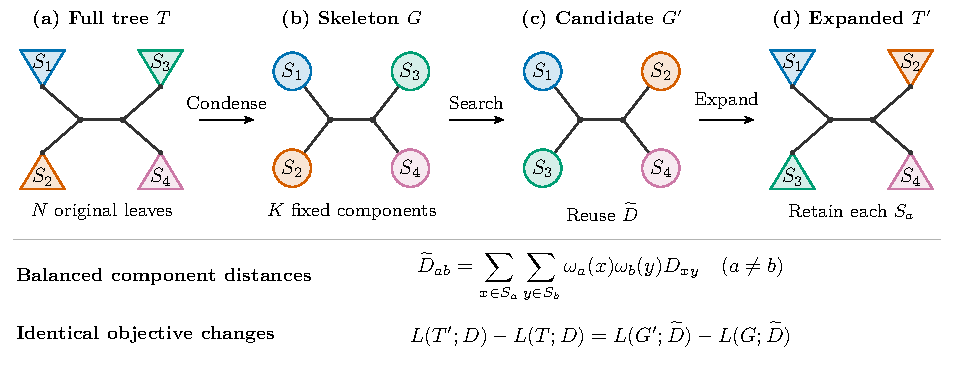
\includegraphics[width=\linewidth]{figures/exact_block_overview.pdf}
 \caption{Block evaluation preserving BME, illustrated with $K=4$ fixed components. \textbf{(a)} Triangles represent components $S_a$ of the full tree, each attached at its apex. \textbf{(b)} Each component becomes one skeleton leaf. The condensed distance $\widetilde D_{ab}$ retains all leaf pairs between $S_a$ and $S_b$, with balanced weights $\omega$ obtained by halving mass at each binary split. \textbf{(c)} Search changes the connections between components while reusing $\widetilde D$. \textbf{(d)} Expanding the candidate preserves each component's internal topology and attachment root. Within-component contributions cancel, so the skeleton and full-tree objective changes agree. A proper subtree window includes its entire complement as an additional component.}
 \label{fig:block_overview}
\end{figure}

\subsection{BME and Phylo2Vec coordinates}
\label{sec:coordinates}

Let $T$ be an unrooted binary tree on $N\geq3$ labeled leaves, and let $D$ be a fixed, finite, symmetric matrix with zero diagonal.
Write $q_T(x,y)$ for the number of internal degree-three vertices on the path from $x$ to $y$.
The BME objective is
\begin{equation}
 L(T;D)=\sum_{0\leq x<y<N}D_{xy}\,2^{-q_T(x,y)}.
 \label{eq:pauplin}
\end{equation}
If the path has $e_T(x,y)$ edges, then $q_T(x,y)=e_T(x,y)-1$.
Thus the unordered-pair coefficient is $2^{1-e_T(x,y)}$.
An artificial degree-two root used to encode the tree is suppressed before evaluating these path lengths.
No additivity assumption on $D$ is needed for the identities below.

The Phylo2Vec domain for rooted binary trees is
\begin{equation}
 \mathcal V_N=\{(v_0,\ldots,v_{N-2}):0\leq v_i\leq2i\},
 \qquad |\mathcal V_N|=(2N-3)!!.
 \label{eq:phylo2vec_space}
\end{equation}
We use the ordered, or cherry-first, subset
$\mathcal V_N^{\mathrm{cf}}=\{v:0\leq v_i\leq i\}$ as the baseline for coordinate evaluation.
Every rooted binary tree can be represented in this subset after a suitable leaf permutation~\cite[Lemmas~0.9--0.11]{penn2023gradme}.
Appendix~\ref{sec:gauge} gives the child-order rule used here.
If $\pi(a)$ is the original leaf represented by current index $a$, the distance matrix in these coordinates is
$D_\pi[a,b]=D[\pi(a),\pi(b)]$.
Permuting both axes in this way preserves the objective.
Constructing the permutation takes $O(N)$ time from a decoded tree, while explicitly copying a dense permuted matrix takes $O(N^2)$ time.

Write $T(v)$ for the unrooted tree obtained by decoding $v$ and suppressing its artificial root.
For an ordered baseline $v$, define the discrete coordinate difference
\begin{equation}
 \Delta_{i,j}
 =L\bigl(T(v^{(i\leftarrow j)});D_\pi\bigr)
  -L\bigl(T(v);D_\pi\bigr),\qquad 0\leq j\leq2i.
 \label{eq:discrete_gradient}
\end{equation}
Here $v^{(i\leftarrow j)}$ replaces only entry $i$ by $j$.
Row $i$ of the table therefore enumerates the allowed replacements of one coordinate, and $\Delta_{i,j}<0$ identifies an improving move.
We use \emph{discrete gradient} as a synonym for this table of finite objective differences, and \emph{coordinate sweep} for one evaluation of the table at a fixed tree.
There are $(N-1)^2$ valid coordinate entries, including unchanged coordinates and entries that can represent the same unrooted topology.
This count is not a count of distinct SPR neighbors.
General candidate values $j>i$ are allowed even though the baseline is ordered.
After accepting such a move, the resulting tree is decoded and relabeled before the next ordered evaluation.
Relabeling changes computational indices and permutes both axes of $D$ together, so the observations remain attached to their original leaves.

\begin{samepage}
\subsection{Quadratic-time coordinate evaluation}

The evaluator first constructs a shared table of subtree distances, then propagates score changes across regraft positions.
For distinct vertices $u,w$, let $A(u,w)$ be the balanced mean distance under $D_\pi$ between the components rooted at $u,w$ and directed away from their connecting path.
If $a,b$ are the two neighbours of an internal vertex $u$ away from $w$, equal weighting of the two branches gives
\begin{equation}
 A(u,w)=\tfrac12\{A(a,w)+A(b,w)\}.
 \label{eq:bottom_up}
\end{equation}
\end{samepage}

For a leaf $x$, initialize $A(y,x)=D_\pi[y,x]$ at the other leaves and apply Equation~\eqref{eq:bottom_up} towards $x$, processing children before their parent.
Each of the $N-2$ internal entries is one average of two previously computed values, so the entire column costs $O(N)$.
Once all leaf columns are complete, symmetry supplies the leaf entries $A(x,w)=A(w,x)$ for each internal target $w$.
The same recurrence computes the entries in its three incident branches in $O(N)$ operations; the diagonal is unused.
Thus all $2N-2$ columns cost $O(N^2)$, including on unbalanced trees.
Appendix~\ref{sec:parallel_details} describes the implementation with a fixed computational root.

For each coordinate $i\geq1$, varying $v_i$ regrafts a fixed subtree $P_i$ (Lemma~\ref{lem:coord_spr}).
Moving its attachment between adjacent edges is a nearest-neighbour interchange (NNI).
For the four components $P,Q,R,S$ surrounding the current NNI edge, let $d_{UV}$ denote the balanced mean distance between $U,V$ at their attachment roots.
The interchange $PQ\mid RS\to PR\mid QS$ changes the BME score by
\begin{equation}
 \delta_{\mathrm{NNI}}=\tfrac14(d_{PR}+d_{QS}-d_{PQ}-d_{RS}).
 \label{eq:nni_increment}
\end{equation}
The standard SPR recurrence accumulates these increments along the remaining tree, obtaining the changing component means from $A$ and a constant number of running averages and weights per traversal state~\cite{hordijk2005spr}.
Each edge therefore costs $O(1)$ operations, and a single traversal scores all regraft positions for $P_i$ in $O(N)$.
The edge-to-coordinate map in Appendix~\ref{sec:mapping} extracts the scores for the $2i+1$ coordinate values.

\begin{proposition}[Quadratic coordinate evaluation]
\label{prop:quadratic}
Given an ordered $N$-leaf encoding $v$, its leaf permutation $\pi$, and constant-time access to $D_\pi$, all $(N-1)^2$ entries in Equation~\eqref{eq:discrete_gradient} can be evaluated using $O(N^2)$ arithmetic operations and $O(N^2)$ storage.
In real arithmetic, every entry equals the corresponding full-tree BME difference.
\end{proposition}
\begin{proof}
Constructing $A$ costs $O(N^2)$.
For each row $i=1,\ldots,N-2$, the SPR traversal and coordinate mapping take $O(N)$ operations, while $\Delta_{0,0}=0$.
The total is therefore
\[
 \underbrace{O(N^2)}_{\text{construct }A}
 +\underbrace{(N-2)\,O(N)}_{\text{evaluate coordinate rows}}
 =O(N^2).
\]
The stored tables have $O(N^2)$ entries.
The SPR recurrence gives changes relative to the original attachment, and the edge map in Appendix~\ref{sec:mapping} identifies them with the corresponding coordinate replacements.
\end{proof}

Every candidate topology is either unchanged or an SPR neighbour; the coordinate table need not cover the full SPR neighbourhood.

\subsection{Condensed distances and BME preservation}
\label{sec:condensation}

Partition all $N$ leaves into $K\geq3$ fixed components $S_1,\ldots,S_K$.
Each component has a fixed internal binary topology and a single attachment to the rest of the tree.
A component can consist of one leaf.
For a non-singleton component, let $r_a$ be the internal vertex adjacent to its attachment edge, and let $h_a(x)$ count the branching vertices from $r_a$ to leaf $x$, including $r_a$.
For a singleton, set $h_a(x)=0$.
Define its balanced leaf weights by
\begin{equation}
 \omega_a(x)=2^{-h_a(x)},\qquad x\in S_a.
 \label{eq:profile}
\end{equation}

The weights sum to one within each component (Lemma~\ref{lem:normalization} in Appendix~\ref{sec:block_proof}).

Let $G$ be an unrooted binary skeleton with one leaf for each component.
Construct $T_G$ by replacing skeleton leaf $a$ with $S_a$, retaining the attachment edge.
Define a condensed distance matrix by
\begin{equation}
 \widetilde D_{ab}
 =\sum_{x\in S_a}\sum_{y\in S_b}
    \omega_a(x)\omega_b(y)D_{xy}\quad(a\ne b),
 \qquad \widetilde D_{aa}=0.
 \label{eq:condensed_D}
\end{equation}
These are exact balanced averages of the original pairwise distances.
They can be formed by the weighted sum above or, equivalently, by recursively averaging over the two children of each component root.
All leaf contributions are retained.
This is an objective-level form of the fixed-clade reduction discussed by Haws et al.~\cite[Section~2.4]{haws2011optimality}.
We include the proof to specify the weights and the scope of exactness needed by the algorithm.

\begin{theorem}[BME decomposition over fixed components]
\label{thm:clade_condense}
There is a constant $C$, independent of the skeleton topology, such that
\begin{equation}
 L(T_G;D)=C+L(G;\widetilde D).
 \label{eq:bme_condense_decomp}
\end{equation}
Consequently, for any two skeletons $G$ and $G'$,
\begin{equation}
 L(T_{G'};D)-L(T_G;D)
 =L(G';\widetilde D)-L(G;\widetilde D).
 \label{eq:condensed_delta}
\end{equation}
\end{theorem}
The proof in Appendix~\ref{sec:block_proof} separates the fixed within-component terms from the between-component terms, whose weights factor through the skeleton.

The constant $C$ contains the contributions of pairs within the same fixed component.
It cancels when comparing skeletons, so the reduction preserves every objective change even though the skeleton's absolute score omits $C$.
The result applies to every reconnection that preserves the components and to arbitrary fixed dissimilarities, including non-additive estimated distances.

\begin{corollary}[Exact minibatch coordinate differences]
\label{cor:minibatch_gradient}
Let $v$ encode an ordered skeleton $G$, keep the attached components fixed, and index $\widetilde D$ by the same leaf labeling.
Evaluating a coordinate replacement $v_i\leftarrow j$ using the exact matrix $\widetilde D$ gives
\begin{equation}
 \Delta^{\mathrm{skel}}_{i,j}
 =L\bigl(T_{G(v^{(i\leftarrow j)})};D\bigr)
  -L\bigl(T_{G(v)};D\bigr).
 \label{eq:minibatch_gradient}
\end{equation}
Once $\widetilde D$ is available, all valid skeleton coordinate differences can be evaluated in $O(K^2)$ time.
\end{corollary}
\begin{proof}
Apply Proposition~\ref{prop:quadratic} to the $K$-leaf skeleton with input $\widetilde D$.
Equation~\eqref{eq:condensed_delta} identifies each resulting skeleton difference with the corresponding full-tree difference.
\end{proof}

\begin{corollary}[A proper subtree window]
\label{cor:outside}
For a window attached to the rest of a binary tree by one edge, treat its entire complement as an additional component oriented away from that edge.
If its internal topology and exact balanced distances to the other components are retained, Equation~\eqref{eq:condensed_delta} applies to rearrangements of the window skeleton.
\end{corollary}
\begin{proof}
Cutting the attachment edge produces two components.
The endpoint in the complement has two outward branches unless the complement is a singleton.
It therefore defines precisely a binary component of the type used in the theorem.
Including it completes the partition of all leaves, so both within-window and window-to-complement contributions are included.
\end{proof}

The outside component retains distances between leaves inside and outside the window.
Deleting the complement would change the objective being optimized.
The weights entering the outside distances are determined by the current topology of the complement and its attachment edge.
They must be updated when a preceding rearrangement changes that topology.

\begin{corollary}[Linear-time BME branch lengths via condensed profiles]
\label{cor:branch_lengths}
At each of the $N-2$ internal vertices $p$ of an unrooted binary tree $T$, let $A_p,B_p,O_p$ denote the three incident subtrees (two child clades and the parent-side complement) with balanced leaf-weight profiles $\omega_{A_p},\omega_{B_p},\omega_{O_p}$, and let $d^B_{XY}(p)=\sum_{x\in X}\sum_{y\in Y}\omega_X(x)\omega_Y(y)D_{xy}$ for $\{X,Y\}\subset\{A_p,B_p,O_p\}$.
Then Pauplin's~\cite{pauplin2000direct} and FastME's~\cite{desper2002fast} balanced minimum-evolution branch length for every edge $e=(u,p)\in E(T)$ (with $u$ corresponding to $A_p$) is given by
\begin{equation}
 \hat\ell(e)=
 \begin{cases}
  \tfrac12\bigl(d^B_{AB}(p)+d^B_{AO}(p)-d^B_{BO}(p)\bigr), & u\text{ is a leaf},\\[4pt]
  \tfrac14\bigl(d^B_{AB}(p)+d^B_{AO}(p)+d^B_{AO}(u)+d^B_{BO}(u)\bigr)
  -\tfrac12\bigl(d^B_{BO}(p)+d^B_{AB}(u)\bigr), & u\text{ is internal},
 \end{cases}
 \label{eq:bme_branch_lengths}
\end{equation}
satisfying $\sum_{e\in E(T)}\hat\ell(e)=L(T;D)$ and requiring only $3(N-2)$ condensed profile-pair evaluations across the entire tree.
\end{corollary}
\begin{proof}
Cutting an internal edge $e=(u,p)$ partitions the leaves into four subtrees $(A_u,B_u)$ on the $u$-side and $(B_p,O_p)$ on the $p$-side, where $A_p=A_u\cup B_u$ and $O_u=B_p\cup O_p$.
By Equation~\eqref{eq:condensed_D}, $d^B(A_p,O_u)=\tfrac12(d^B_{AB}(p)+d^B_{AO}(p))=\tfrac12(d^B_{AO}(u)+d^B_{BO}(u))$, which reduces Pauplin's four-subtree formula $\tfrac14\sum_{X\in\{A_u,B_u\}}\sum_{Y\in\{B_p,O_p\}}d^B(X,Y)-\tfrac12\bigl(d^B_{AB}(u)+d^B_{BO}(p)\bigr)$ to Equation~\eqref{eq:bme_branch_lengths}.
Constructing $\omega_{A_p},\omega_{B_p}$ in one bottom-up post-order pass and $\omega_{O_p}$ in one top-down pre-order pass evaluates all $2N-3$ branch lengths from the $3(N-2)$ node-local pairs $\bigl(d^B_{AB}(p),d^B_{AO}(p),d^B_{BO}(p)\bigr)$.
\end{proof}

\subsection{Minibatch evaluation and sequential updates}
\label{sec:acceptance}

With the fixed components and exact condensed matrix in place, candidate skeletons are evaluated against the full-tree objective through Corollary~\ref{cor:minibatch_gradient}.
The same matrix can be reused throughout a skeleton search because its component topologies and attachment roots remain fixed.
For a candidate $G'$, let $\mathcal P(G,G')=\{(a,b):a<b,\ q_G(a,b)\ne q_{G'}(a,b)\}$.
Its full-tree BME change can also be computed directly from the changed pairs:
\begin{equation}
 \delta=\sum_{(a,b)\in\mathcal P(G,G')}
   \left(2^{-q_{G'}(a,b)}-2^{-q_G(a,b)}\right)
   \widetilde D_{ab}.
 \label{eq:changed_pairs}
\end{equation}
Unchanged pairs contribute zero, and the within-component constant cancels.
Theorem~\ref{thm:clade_condense} therefore identifies $\delta$ with the full-tree BME change.
Thus both coordinate selection and the evaluation of a combined candidate can use the same exact condensed distances.

Windows are committed sequentially.
After a commit, affected ancestor summaries are updated and the next window's outside distances are constructed from the current tree.
Node-disjoint windows need not have additive BME changes because both updates can alter the coefficients of distances between their leaves.
For consecutive accepted trees $T^{(0)},\ldots,T^{(M)}$, exact arithmetic gives
\begin{equation}
 L(T^{(M)};D)-L(T^{(0)};D)
 =\sum_{m=1}^M\bigl[L(T^{(m)};D)-L(T^{(m-1)};D)\bigr].
 \label{eq:telescoping}
\end{equation}
If each increment is negative, so is the cumulative increment.
This argument requires that each acceptance calculation uses the current tree, rather than a shared pre-update tree.

On sufficiently deep trees, finite-precision leaf weights can also underflow.

\subsection{Optimisation algorithm}
\label{sec:optimizer}

Algorithm~\ref{alg:block_search} separates block construction from candidate search.
Its inputs are a starting tree $T_0$, fixed distances $D$, a schedule $\mathcal W$, and a skeleton solver $\mathcal A$.
$\proc{Skeleton}$ returns a partition $\mathcal S$ of all leaves into fixed rooted components and their current skeleton $G$.
For a proper subtree window, $\mathcal S$ includes the entire oriented complement.
$\proc{Weights}$ constructs their balanced weights $\Omega=\{(S_a,\omega_a)\}_{a=1}^K$.
$\proc{Condense}$ evaluates Equation~\eqref{eq:condensed_D} without truncation, and $\proc{Expand}$ restores the same components with their original leaf identities.
The components and their attachment roots remain fixed during each solver call.
Full-tree search is the special case of one block containing $N$ singleton components.

\begin{algorithm}[!htbp]
\caption{Full-tree and minibatch BME search}
\label{alg:block_search}
\small
\textbf{Input:} $T_0$, $D$, schedule $\mathcal W$, solver $\mathcal A$, block and sweep budgets $B,I$, margin $\varepsilon\geq0$.\par
\textbf{Output:} tree $T$ and accumulated score change $s$.\par\smallskip
\begin{tabular*}{\linewidth}{@{}r@{\quad}>{\raggedright\arraybackslash}p{.74\linewidth}@{\extracolsep{\fill}}r@{}}
  & & \textsf{Execution}\\
1 & $T\gets T_0$; $s\gets0$ & \onCPU\\
2 & \textbf{for} $b=0,\ldots,B-1$ \textbf{do} & \onCPU\\
3 & \algindent{1}$w\gets\mathcal W(T,b)$; \textbf{if} $w=\bot$ \textbf{then break} & \onCPU\\
4 & \algindent{1}$(G,\mathcal S)\gets\proc{Skeleton}(T,w)$ & \onCPU\\
5 & \algindent{1}$\Omega\gets\proc{Weights}(\mathcal S)$ & \onCPU\\
6 & \algindent{1}$M\gets\proc{Condense}(\Omega,D)$ & \onGPU\\
7 & \algindent{1}$G'\gets\mathcal A(G,M;I)$ & \onBoth\\
8 & \algindent{1}$\delta\gets L(G';M)-L(G;M)$ & \onBoth\\
9 & \algindent{1}\textbf{if} $\delta<-\varepsilon$ \textbf{then} & \onCPU\\
10 & \algindent{2}$T\gets\proc{Expand}(G',\mathcal S)$; $s\gets s+\delta$ & \onCPU\\
11 & \algindent{2}$\proc{Refresh}(T)$ & \onCPU\\
12 & \textbf{return} $(T,s)$ & \onCPU\\
\end{tabular*}
\par\smallskip
{\footnotesize Execution labels refer to the GPU implementation. \onBoth{} denotes a mixed stage.}
\end{algorithm}

Each block is constructed from the current tree.
$\proc{Refresh}$ updates affected ancestor summaries, and outside distances are rebuilt before the next window.
The acceptance test evaluates the joint candidate, including interactions between its coordinate updates.
By Theorem~\ref{thm:clade_condense}, every committed change decreases the full-tree objective in real arithmetic.
A schedule may expose overlapping local windows and larger backbone connections. Its construction and implementation parameters are specified in Appendix~\ref{sec:search_policies}.

Algorithm~\ref{alg:coordinate_search} gives the CPU skeleton solver.
The persistent state $(v,\pi)$ contains the encoding and its map to original component identities, with $M_\pi[a,b]=M[\pi(a),\pi(b)]$.
$\proc{Normalise}$ leaves an ordered encoding unchanged and otherwise relabels it, composing the permutation.
$\proc{Sweep}$ returns the current score and coordinate differences. $\proc{RankMin}$ sorts the improving row minima.
$\proc{BatchStep}$ tests compatible batches by their joint score, halves a rejected batch, and falls back to the best single move.
$\proc{Best}$ selects the lower-scoring tree, retaining its first argument on a tie.

\begin{algorithm}[!htbp]
\caption{CPU skeleton search}
\label{alg:coordinate_search}
\small
\textbf{Input:} $G_0$, component matrix $M$, sweep and escape budgets $I,E$, margin rule $\epsilon(\ell)$.\par
\textbf{Output:} best scored skeleton in its original component labeling.\par\smallskip
\begin{tabular}{@{}r@{\quad}>{\raggedright\arraybackslash}p{.93\linewidth}@{}}
1 & $(v,\pi)\gets\proc{Order}(G_0)$; $G_\star\gets G_0$; $r\gets0$; $e\gets0$\\
2 & \textbf{for} $t=1,\ldots,I$ \textbf{do}\\
3 & \algindent{1}$(v,\pi)\gets\proc{Normalise}(v,\pi)$\\
4 & \algindent{1}$(\ell,\Delta)\gets\proc{Sweep}(v,M_\pi)$; $\eta\gets\epsilon(\ell)$\\
5 & \algindent{1}$G_\star\gets\proc{Best}(G_\star,\proc{Decode}(v,\pi);M)$\\
6 & \algindent{1}$R\gets\proc{RankMin}(\Delta,-\eta)$\\
7 & \algindent{1}\textbf{if} $R\ne\varnothing$ \textbf{then}\\
8 & \algindent{2}$v\gets\proc{BatchStep}(v,M_\pi,R,\eta)$; $r\gets0$; \textbf{continue}\\
9 & \algindent{1}$u\gets\proc{ExtraSPR}(v,M_\pi,\eta)$\\
10 & \algindent{1}\textbf{if} $u=\bot$ \textbf{and} $r=0$ \textbf{then}\\
11 & \algindent{2}$(v,\pi)\gets\proc{Reverse}(v,\pi)$; $r\gets1$; \textbf{continue}\\
12 & \algindent{1}\textbf{if} $u=\bot$ \textbf{then} $u\gets\proc{RemainingSPR}(v,M_\pi,\eta)$\\
13 & \algindent{1}\textbf{if} $u=\bot$ \textbf{and} $e<E$ \textbf{and} $t<I$ \textbf{then}\\
14 & \algindent{2}$e\gets e+1$; $u\gets\proc{Escape}(v,\Delta,e,\eta)$\\
15 & \algindent{1}\textbf{if} $u=\bot$ \textbf{then break}\\
16 & \algindent{1}$v\gets u$; $r\gets0$\\
17 & \textbf{return} $\proc{Best}(G_\star,\proc{Decode}(v,\pi);M)$\\
\end{tabular}
\end{algorithm}

Here $\bot$ denotes failure to find a candidate, and $r$ records whether the reversed ordered labeling has been tried since the last topology change.
$\proc{ExtraSPR}$ checks additional regrafts for the pruned components already scanned, while $\proc{RemainingSPR}$ completes the unrooted SPR scan, including complement-side prunes.
Both require a change below $-\eta$.
$\proc{Reverse}$ changes the ordered labeling and composes $\pi$ without changing the tree.
$\proc{Escape}$ proposes a deterministic pair of uphill coordinate replacements, with the best scored tree retained across such trials.
Appendix~\ref{sec:search_policies} defines the batch and escape rules.

The GPU solver is an alternative $\mathcal A$.
Balanced-distance recurrences, row-minimum evaluation, and score reductions run on the GPU.
The CPU packs the SPR proposals, updates and relabels the tree, and retains the best scored skeleton without the CPU completion scan.
For the block change, the GPU supplies scores or pair-distance contributions and the CPU assembles the final difference and decides acceptance.
The objective-preservation guarantee requires complete distances for acceptance and current outside information.
A block or sweep budget limits the search, and only a completed unsuccessful SPR scan establishes SPR-local optimality up to the numerical margin.
Neither solver guarantees a global BME optimum.

\subsection{Parallel evaluation and computational cost}
\label{sec:parallel}

Equation~\eqref{eq:bottom_up} has an independent recurrence for each fixed column.
Assigning columns to threads lets neighboring threads access consecutive entries while following the same traversal order.
The top-down correction for column $w$ follows its ancestor path.
Depth-first entry intervals determine the next child without a traversal stack.
Its total work over columns is $O(\sum_w\operatorname{depth}(w))$, bounded by $O(N^2)$ and reduced to $O(N\log N)$ for trees of logarithmic height.

A full balanced-distance table stores approximately $4N^2$ entries.
The column-tiled variant retains the internal-to-leaf block and reconstructs required internal rows on demand.
This reduces that table to approximately $N^2$ entries, while the input matrix and other buffers still contribute to total memory.
A row-wise reduction can return the best coordinate replacement in each row without storing the full coordinate table.
Columns and SPR rows can also be distributed across GPUs.
Appendix~\ref{sec:parallel_details} gives the dependency and workspace arguments.

For a skeleton with $K$ leaves, a coordinate sweep costs $O(K^2)$ once its distances are available.
This does not make arbitrary distance construction independent of $N$.
Direct evaluation of one condensed pair can require $|S_a||S_b|$ original distances.
Explicit leaf weights use $O(N)$ entries, and constructing exact condensed distances can dominate runtime for large component pairs.
When $D_{xy}=\phi(x)^\top\psi(y)$ has a fixed-dimensional bilinear representation, weighted component embeddings give
$\widetilde D_{ab}=(\sum_x\omega_a(x)\phi(x))^\top
(\sum_y\omega_b(y)\psi(y))$.
That shortcut is exact for the specified bilinear distance.
It does not justify averaging embeddings before applying a nonlinear sequence-distance correction.

\section{Experimental design}
\label{sec:experiments}

We evaluate sequence-to-tree refinement from $N=1{,}000$ to $N=10{,}000{,}000$ leaves across two simulated benchmark suites with known reference topologies:
\begin{enumerate}
 \item \textbf{RNASim ($L=1{,}596$ sites).} Subsampled alignments from the million-taxon RNASim simulation benchmark~\cite{mirarab2015pasta} at $N=1{,}000$, $5{,}000$, $10{,}000$, $50{,}000$, $100{,}000$, $1{,}000{,}000$, and a $10{,}000{,}000$-leaf extension.
 \item \textbf{Jukes--Cantor ($L=10{,}000$ and $L=1{,}000$ sites).} Unpaginated DNA alignments simulated under the Jukes--Cantor model at $L=10{,}000$ sites (\texttt{JC10k}) across $N=1{,}000$ to $10{,}000{,}000$ leaves, paired with $L=1{,}000$-site alignments (\texttt{JC1k}) at $N=10{,}000$ to isolate the effect of sequence length on distance noise and topological recovery.
\end{enumerate}

For $N\leq100{,}000$, every condition is evaluated over $R=5$ independent replicates ($\text{rep}=0,\ldots,4$), reporting mean and standard deviation across replicates.
At $N=1{,}000{,}000$ and $10{,}000{,}000$, single-replicate runs are reported due to baseline compute cost.
All refinement methods at $N\leq1{,}000{,}000$ start from the same initial tree produced by VeryFastTree~4.0.5~\cite{pineiro2020veryfasttree} with minimum-evolution and maximum-likelihood phases disabled (\texttt{VFT-InitNJ}, flags \texttt{-nome -noml}).
At $N=10{,}000{,}000$, where constructing a full neighbor-joining starting tree is prohibitive, refinement starts from a perturbed reference tree with initial normalized Robinson--Foulds (RF) error of approximately $35.9\%$.

We compare GPU full-tree search (\texttt{Phylo2Vec-Full}, evaluated up to $N=10{,}000$) and GPU minibatch search (\texttt{Phylo2Vec-Minibatch}, evaluated up to $N=10{,}000{,}000$) under gap-aware Jukes--Cantor (JC69) distances against both 64-thread CPU baselines---FastME~2.1.6 SPR refinement (\texttt{-s})~\cite{lefort2015fastme}, FastTreeMP~2.2~\cite{price2010fasttree} and VeryFastTree~4.0.5 minimum-evolution refinement (\texttt{-noml}), and reference maximum-likelihood refinement (\texttt{ME+ML}, evaluated up to $N=10{,}000$)---and the GPU distance-based phylogenetic placer DIPPER~0.1.5~\cite{walia2026dipper} (\texttt{-i m -o t -d 2 --force-binary}, evaluated up to $N=1{,}000{,}000$, which constructs trees directly from sequences on GPU via neighbor-joining for $N<30{,}000$, $K$-closest placement for $30{,}000\leq N<1{,}000{,}000$, and divide-and-conquer placement at $N=1{,}000{,}000$).
For trees above $2{,}048$ leaves, the sequence minibatch implementation caps component leaf-weight lists at 64 entries during inner skeleton proposals and recomputes all affected condensed pairs over complete leaf profiles before evaluating Equation~\eqref{eq:changed_pairs} in FP64 (acceptance margin $10^{-6}$).
At $N=10{,}000{,}000$, packed two-bit sequences are streamed from disk to GPU memory in 256~MB chunks to bound host memory usage.

We record four metrics for every run: topological error measured by normalized RF distance (incorrect nontrivial splits divided by $N-3$), wall-clock refinement time (excluding the shared \texttt{VFT-InitNJ} initialization), BME objective change $\Delta\text{BME}$ relative to the starting tree under the exact full-tree JC69 distance matrix, and peak memory footprint (maximum resident set size on the host CPU and peak allocated device memory on the GPU).
Independent numerical verification of the coordinate evaluator, small-tree CPU comparisons, and standalone multi-GPU sweep microbenchmarks are reported in Appendix~\ref{sec:additional_results}.

\section{Results}
\label{sec:results}

Figures~\ref{fig:rnasim_scaling} and~\ref{fig:jc_scaling_4panel} summarize runtime scaling, topological accuracy, peak memory footprint, and sequence-length sensitivity across the RNASim ($L=1{,}596$) and Jukes--Cantor ($L=1{,}000$ and $10{,}000$) benchmarks from $N=1{,}000$ to $10{,}000{,}000$ leaves (complete numerical tables in Appendix~\ref{sec:additional_results}).

\begin{figure*}[tbp]
 \centering
 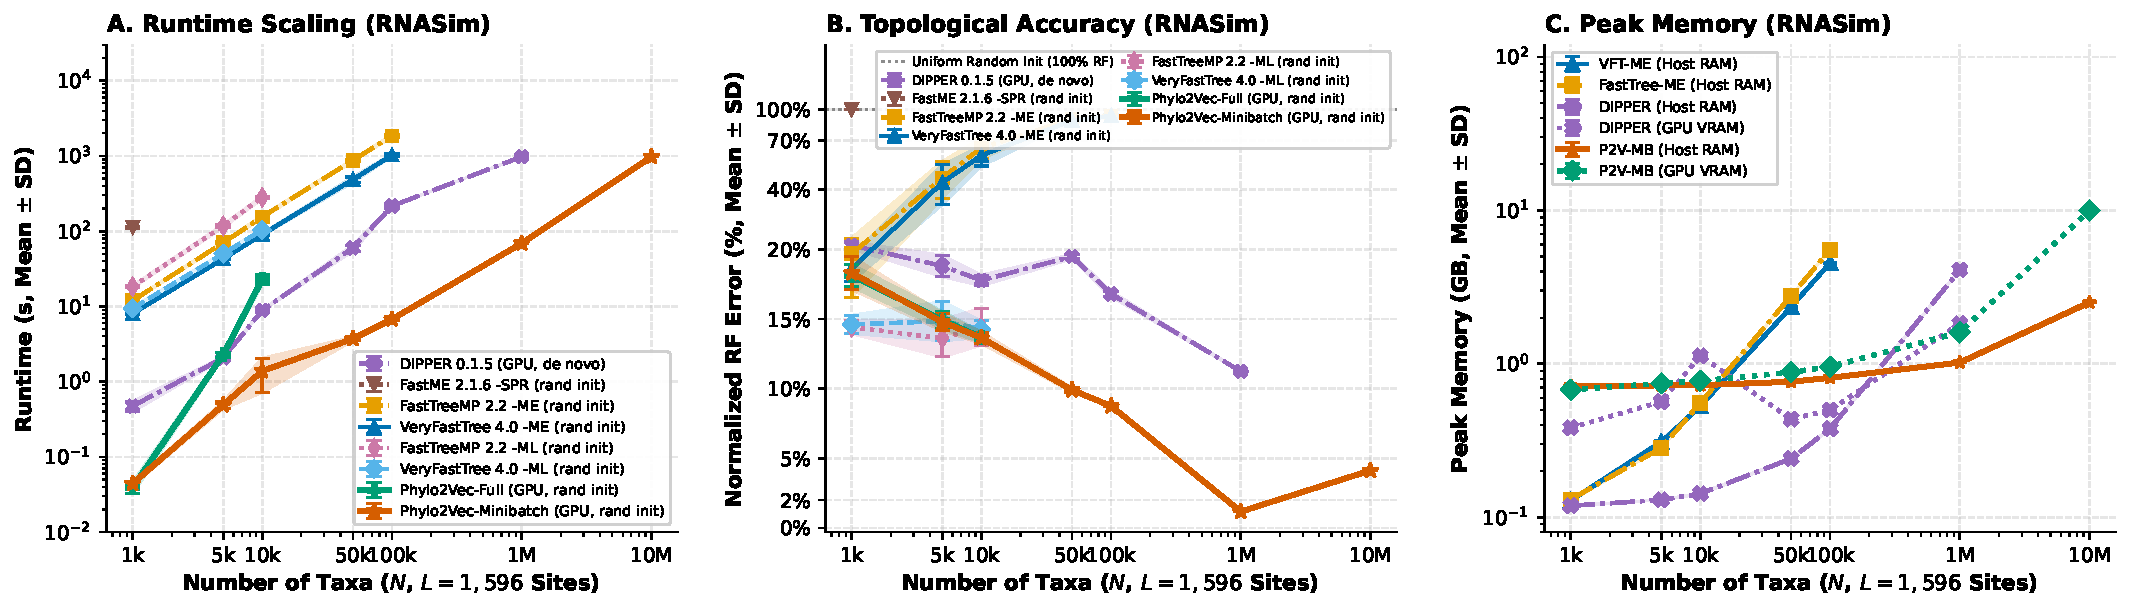
\includegraphics[width=\textwidth]{figures/paper1_rnasim_scaling_figure.pdf}
 \caption{Sequence-to-tree refinement scaling on simulated \textbf{RNASim} alignments ($L=1{,}596$ sites) across $N=1{,}000$ to $10{,}000{,}000$ leaves ($R=5$ independent replicates for $N\leq100{,}000$; points and error bars show $\text{mean}\pm1\text{ SD}$). \textbf{(A)} Wall-clock refinement runtime. \textbf{(B)} Normalized Robinson--Foulds topological error (\%). \textbf{(C)} Peak host RAM and GPU VRAM footprint.}
 \label{fig:rnasim_scaling}
\end{figure*}

\begin{figure*}[tbp]
 \centering
 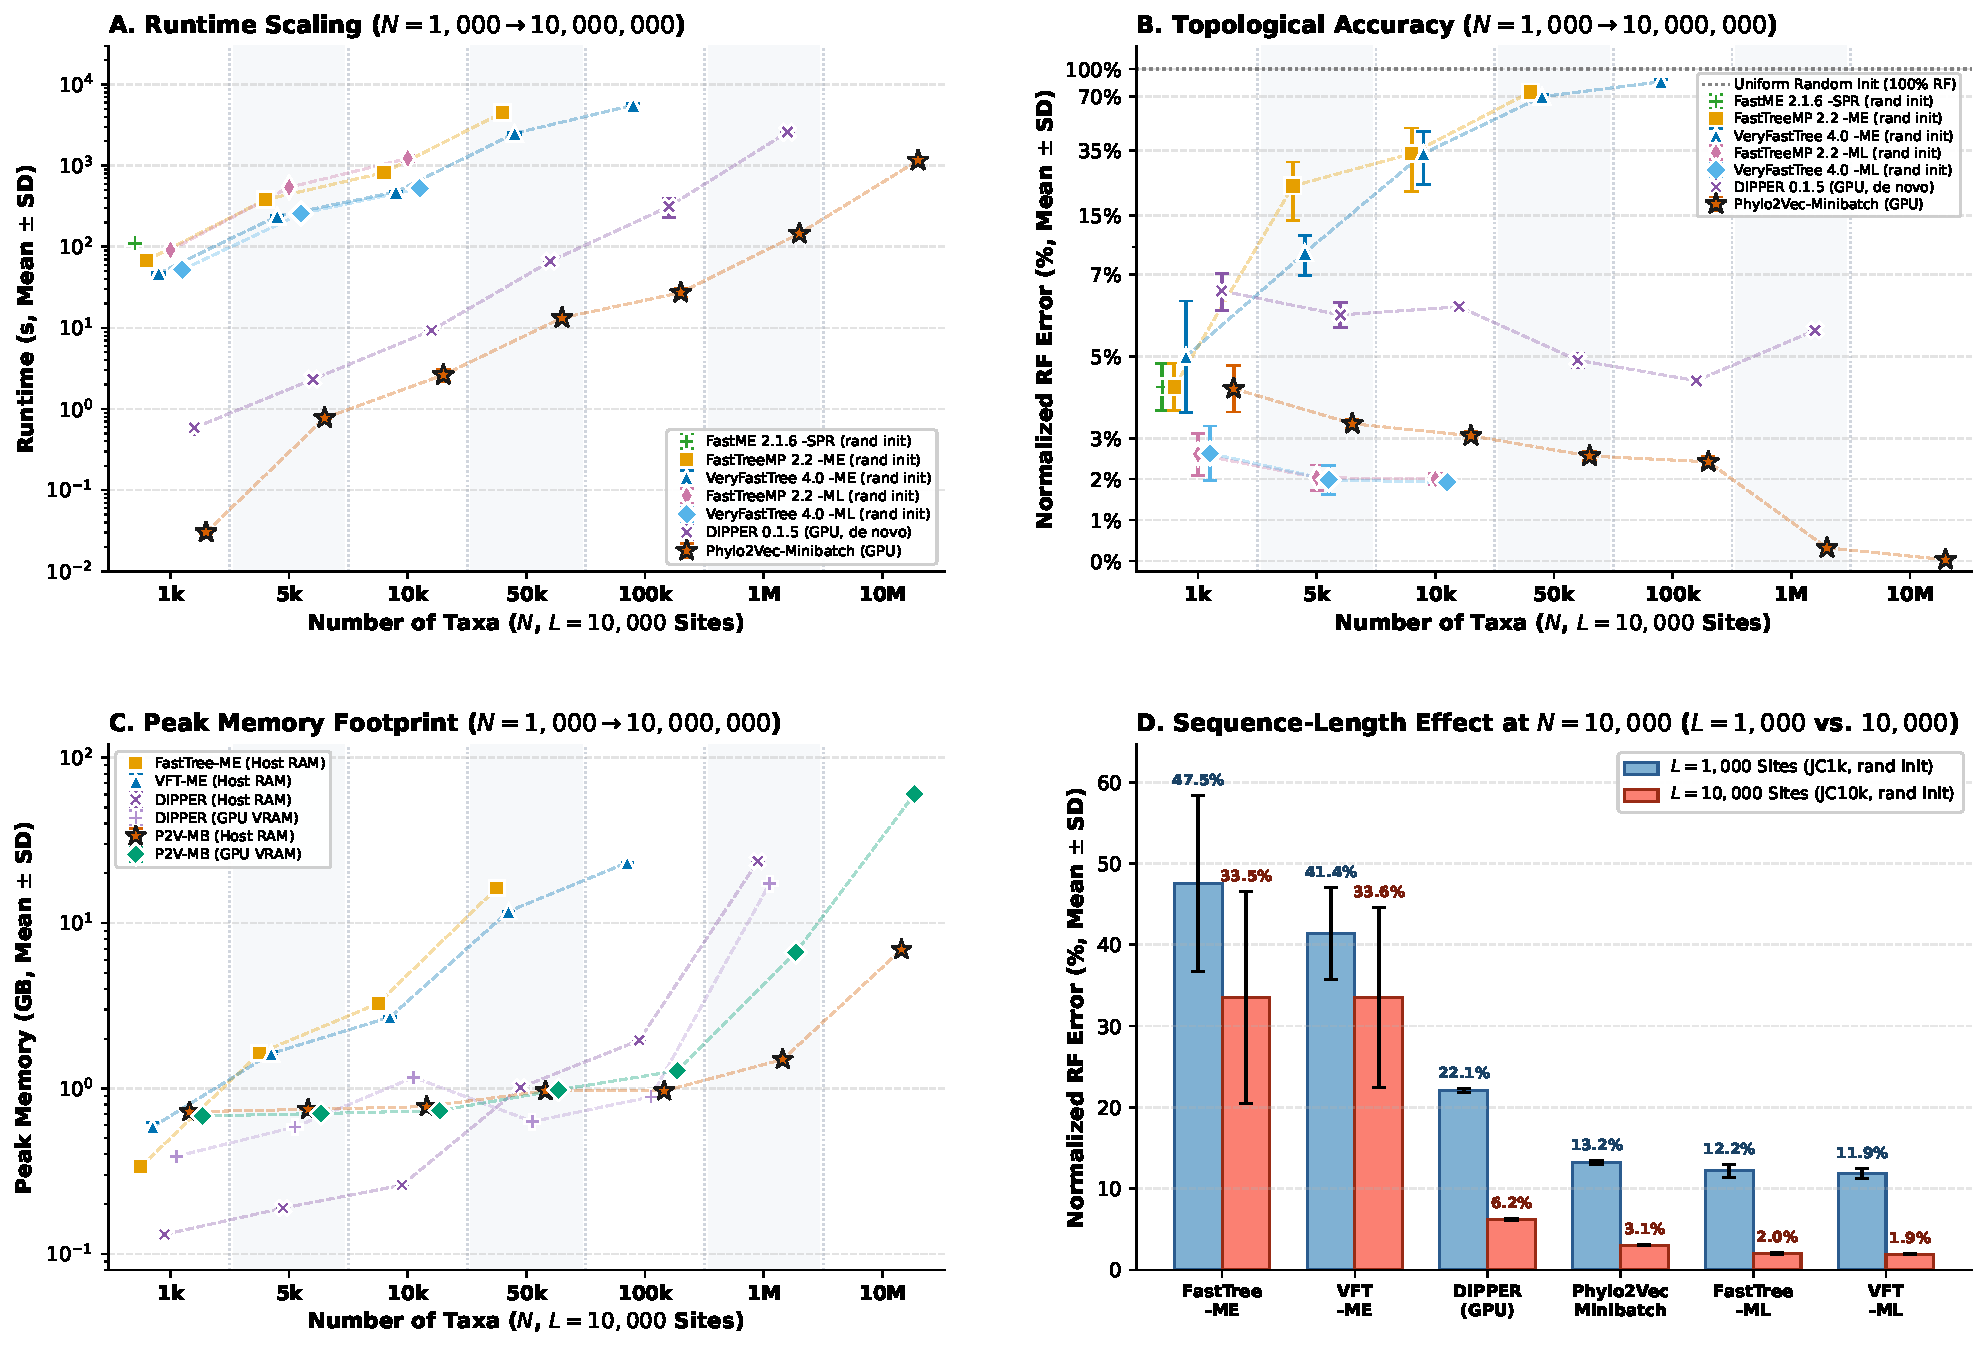
\includegraphics[width=\textwidth]{figures/paper1_jc_scaling_figure.pdf}
 \caption{Sequence-to-tree refinement scaling on simulated \textbf{Jukes--Cantor} alignments across $N=1{,}000$ to $10{,}000{,}000$ leaves ($R=5$ independent replicates for $N\leq100{,}000$; points and error bars show $\text{mean}\pm1\text{ SD}$). \textbf{(A)} Wall-clock refinement runtime on $L=10{,}000$-site alignments (\texttt{JC10k}). \textbf{(B)} Normalized Robinson--Foulds topological error (\%) on \texttt{JC10k}. \textbf{(C)} Peak host RAM and GPU VRAM footprint across $N=1{,}000$ to $10{,}000{,}000$. \textbf{(D)} Effect of sequence length ($L=1{,}000$ vs.\ $L=10{,}000$ sites) on topological accuracy at $N=10{,}000$ leaves.}
 \label{fig:jc_scaling_4panel}
\end{figure*}

Three consistent trends emerge across both benchmark suites:
\begin{enumerate}
 \item \textbf{Global convergence from uniform random trees.} Starting from uniform random topologies ($100.0\%$ initial RF error), CPU minimum-evolution local searches (\texttt{FastTreeMP -noml -intree} and \texttt{VeryFastTree -noml -intree}) become trapped in poor local optima as $N$ grows ($70.0\text{--}84.9\%$ RF error on \texttt{JC10k} and $88.1\text{--}92.7\%$ on \texttt{RNASim} at $N=50{,}000\text{--}100{,}000$), whereas \texttt{Phylo2Vec-Minibatch} recovers global topology down to $2.45\text{--}2.61\%$ RF on \texttt{JC10k} ($1.40\%$ at $N=10^6$ and $2.58\%$ at $N=10^7$) and $8.76\text{--}9.91\%$ RF on \texttt{RNASim} ($1.17\%$ at $N=10^6$ and $4.13\%$ at $N=10^7$), outperforming \textit{de novo} GPU placement (\texttt{DIPPER 0.1.5}) across every dataset and regime (Figures~\ref{fig:rnasim_scaling}B and~\ref{fig:jc_scaling_4panel}B; Tables~\ref{tab:rnasim_scaling}--\ref{tab:jc10k_scaling}).
 \item \textbf{Runtime, memory, and $O(N)$ branch-length scaling to $10^7$ leaves.} \texttt{Phylo2Vec-Minibatch} decouples the inner sweep cost from $N$, delivering $130\text{--}260\times$ speedups over 64-thread CPU baselines at $N=50{,}000\text{--}100{,}000$ ($3.7\text{--}6.8$~s on \texttt{RNASim}; $13.2\text{--}21.5$~s on \texttt{JC10k}) and refining $N=1{,}000{,}000$ leaves in $1.15\text{--}2.95$~min and $N=10{,}000{,}000$ leaves in $16.2\text{--}31.5$~min on $8\times\text{H100}$ GPUs (Figures~\ref{fig:rnasim_scaling}A and~\ref{fig:jc_scaling_4panel}A). Following topology optimization, Corollary~\ref{cor:branch_lengths} estimates all $2N-3$ FastME/BME branch lengths in $O(N)$ profile evaluations, taking $0.89\text{--}1.00$~s at $N=1{,}000{,}000$ ($0.12\text{--}0.20$~s GPU kernel) and $10.50\text{--}13.33$~s at $N=10{,}000{,}000$ ($1.39\text{--}2.00$~s GPU kernel across $19{,}999{,}997$ edges; Table~\ref{tab:bme_bl_scaling}). Streaming packed sequences into device memory keeps host RAM below $1.9$~GB up to $N=10^6$ and $2.8$~GB at $N=10^7$ (Figures~\ref{fig:rnasim_scaling}C and~\ref{fig:jc_scaling_4panel}C).
 \item \textbf{Effect of sequence length on distance noise.} Increasing alignment length tenfold from $L=1{,}000$ (\texttt{JC1k}) to $L=10{,}000$ (\texttt{JC10k}) reduces the variance of pairwise distance estimates, lowering minimum-evolution RF error more than fourfold ($13.25\%\to3.07\%$ at $N=10{,}000$) and narrowing the topological gap to full maximum-likelihood refinement while retaining a $>160\times$ runtime advantage (Figure~\ref{fig:jc_scaling_4panel}D).
\end{enumerate}

\section{Discussion}

The method separates the size of a search block from the objective it evaluates.
A skeleton can optimize connections among $K$ components while retaining the contribution of every original leaf through balanced component distances.
The same quadratic coordinate evaluator therefore supports both full-tree sweeps ($N\leq10{,}000$) and restricted minibatch searches up to $N=10{,}000{,}000$ leaves.

Across both the RNASim and Jukes--Cantor benchmarks, GPU full-tree and minibatch refinement achieve the same or slightly lower topological error and lower BME objective scores than 64-thread minimum-evolution baselines (\texttt{FastME}, \texttt{FastTree-ME}, and \texttt{VeryFastTree-ME}) and substantially lower topological error than unrefined GPU placement (\texttt{DIPPER}), while reducing refinement wall-clock time from hours to seconds or minutes.
Streaming packed sequence data into device memory avoids large host allocations, enabling ten-million-leaf refinement with $10{,}000$ sites on a single 141~GB H200 GPU using less than $2.2$~GB of host RAM.

Three scope considerations apply to these results.
First, the tested relabeling and block schedules are heuristic and do not guarantee global BME optimality, and the number of sweeps depends on the starting topology.
Second, under finite alignment lengths, minimum evolution optimizes estimated pairwise distances rather than sequence likelihood; as shown in Figure~\ref{fig:jc_scaling_4panel}D, longer alignments reduce distance estimation noise and narrow the gap between minimum-evolution and maximum-likelihood topologies.
Third, for $N>2{,}048$, the sequence minibatch implementation uses capped component profiles to accelerate inner skeleton proposals before verifying candidate blocks against complete leaf profiles in FP64 (Appendix~\ref{sec:search_policies}).

\section{Conclusion}

Shared coordinate evaluation and exact component reduction give a common basis for full-tree and block BME search.
A quadratic sweep evaluates all valid coordinate updates, and the same computation on an exactly condensed skeleton preserves their full-tree objective changes.
The resulting parallel algorithms let a search trade the scope of its candidate set against evaluation cost while retaining the specified BME objective.

\begin{thebibliography}{10}

\bibitem{pauplin2000direct}
Y.~Pauplin.
\newblock Direct calculation of a tree length using a distance matrix.
\newblock \emph{Journal of Molecular Evolution}, 51(1):41--47, 2000.

\bibitem{desper2002fast}
R.~Desper and O.~Gascuel.
\newblock Fast and accurate phylogeny reconstruction algorithms based on the minimum-evolution principle.
\newblock \emph{Journal of Computational Biology}, 9(5):687--705, 2002.

\bibitem{desper2004theory}
R.~Desper and O.~Gascuel.
\newblock Theoretical foundation of the balanced minimum evolution method of phylogenetic inference and its relationship to weighted least-squares tree fitting.
\newblock \emph{Molecular Biology and Evolution}, 21(3):587--598, 2004.
\newblock \href{https://doi.org/10.1093/molbev/msh049}{doi:10.1093/molbev/msh049}.

\bibitem{hordijk2005spr}
W.~Hordijk and O.~Gascuel.
\newblock Improving the efficiency of {SPR} moves in phylogenetic tree search methods based on maximum likelihood.
\newblock \emph{Bioinformatics}, 21(24):4338--4347, 2005.
\newblock \href{https://doi.org/10.1093/bioinformatics/bti713}{doi:10.1093/bioinformatics/bti713}.

\bibitem{lefort2015fastme}
V.~Lefort, R.~Desper, and O.~Gascuel.
\newblock {FastME 2.0}: A comprehensive, accurate, and fast distance-based phylogeny inference program.
\newblock \emph{Molecular Biology and Evolution}, 32(10):2798--2800, 2015.

\bibitem{penn2024phylo2vec}
M.~J.~Penn, N.~Scheidwasser, M.~P.~Khurana, D.~A.~Duch\^ene, C.~A.~Donnelly, and S.~Bhatt.
\newblock {Phylo2Vec}: a vector representation for binary trees.
\newblock \emph{Systematic Biology}, 74(2):250--266, 2025. Advance access 2024.
\newblock \href{https://doi.org/10.1093/sysbio/syae030}{doi:10.1093/sysbio/syae030}.

\bibitem{penn2023gradme}
M.~J.~Penn, N.~Scheidwasser, J.~Penn, C.~A.~Donnelly, D.~A.~Duch\^ene, and S.~Bhatt.
\newblock Leaping through tree space: continuous phylogenetic inference for rooted and unrooted trees.
\newblock \emph{Genome Biology and Evolution}, 15(12):evad213, 2023.
\newblock \href{https://doi.org/10.1093/gbe/evad213}{doi:10.1093/gbe/evad213}.
\newblock Lemma numbers refer to the appendix of \href{https://arxiv.org/abs/2306.05739v4}{arXiv:2306.05739v4}.

\bibitem{tapo2026parallel}
C.~Tapo and Q.~Zhu.
\newblock Parallel and scalable balanced minimum evolution algorithm for large-scale phylogenetic inference.
\newblock \emph{bioRxiv}, 2026. Preprint.
\newblock \href{https://doi.org/10.64898/2026.07.27.740982}{doi:10.64898/2026.07.27.740982}.

\bibitem{camerota2026learning}
F.~J.~Camerota Verd\`u, A.~Gasparin, L.~Bortolussi, and L.~Castelli.
\newblock Learning to explore tree neighbourhoods for phylogenetic inference.
\newblock \emph{Briefings in Bioinformatics}, 27(1):bbaf732, 2026.
\newblock \href{https://doi.org/10.1093/bib/bbaf732}{doi:10.1093/bib/bbaf732}.

\bibitem{haws2011optimality}
D.~C.~Haws, T.~L.~Hodge, and R.~Yoshida.
\newblock Optimality of the neighbor joining algorithm and faces of the balanced minimum evolution polytope.
\newblock \emph{Bulletin of Mathematical Biology}, 73(11):2627--2648, 2011.
\newblock \href{https://doi.org/10.1007/s11538-011-9640-x}{doi:10.1007/s11538-011-9640-x}.

\bibitem{mirarab2015pasta}
S.~Mirarab, N.~Nguyen, S.~Guo, L.-S.~Wang, J.~Kim, and T.~Warnow.
\newblock {PASTA}: ultra-large multiple sequence alignment for nucleotide and amino-acid sequences.
\newblock \emph{Journal of Computational Biology}, 22(5):377--386, 2015.
\newblock \href{https://doi.org/10.1089/cmb.2014.0156}{doi:10.1089/cmb.2014.0156}.

\bibitem{price2010fasttree}
M.~N.~Price, P.~S.~Dehal, and A.~P.~Arkin.
\newblock {FastTree 2}---approximately maximum-likelihood trees for large alignments.
\newblock \emph{PLOS ONE}, 5(3):e9490, 2010.
\newblock \href{https://doi.org/10.1371/journal.pone.0009490}{doi:10.1371/journal.pone.0009490}.

\bibitem{pineiro2020veryfasttree}
C.~Pi\~neiro, J.~M.~Abu\'in, and J.~C.~Pichel.
\newblock {VeryFastTree}: speeding up the estimation of phylogenies for large alignments through parallelization and vectorization.
\newblock \emph{Bioinformatics}, 36(17):4658--4659, 2020.
\newblock \href{https://doi.org/10.1093/bioinformatics/btaa582}{doi:10.1093/bioinformatics/btaa582}.

\bibitem{walia2026dipper}
S.~Walia, Z.~Chen, Y.-H.~Tseng, and Y.~Turakhia.
\newblock Ultrafast and ultralarge distance-based phylogenetics using {DIPPER}.
\newblock \emph{Nature Computational Science}, 2026.
\newblock \href{https://doi.org/10.1038/s43588-026-01015-8}{doi:10.1038/s43588-026-01015-8}.

\bibitem{demaio2023maple}
N.~De~Maio, P.~Kalaghatgi, Y.~Turakhia, R.~Corbett-Detig, B.~Q.~Minh, and N.~Goldman.
\newblock Maximum likelihood pandemic-scale phylogenetics.
\newblock \emph{Nature Genetics}, 55(5):746--752, 2023.
\newblock \href{https://doi.org/10.1038/s41588-023-01368-0}{doi:10.1038/s41588-023-01368-0}.

\bibitem{lytrong2024cmaple}
N.~Ly-Trong, G.~Naseri, N.~De~Maio, and B.~Q.~Minh.
\newblock {CMAPLE}: High-performance maximum-likelihood phylogenetics for pandemic-scale data.
\newblock \emph{Molecular Biology and Evolution}, 41(7):msae134, 2024.
\newblock \href{https://doi.org/10.1093/molbev/msae134}{doi:10.1093/molbev/msae134}.

\bibitem{quast2013silva}
C.~Quast, E.~Pruesse, P.~Yilmaz, J.~Gerken, T.~Schweer, P.~Yarza, J.~Peplies, and F.~O.~Gl\"ockner.
\newblock The {SILVA} ribosomal {RNA} gene database project: improved data processing and web-based tools.
\newblock \emph{Nucleic Acids Research}, 41(D1):D590--D596, 2013.
\newblock \href{https://doi.org/10.1093/nar/gks1219}{doi:10.1093/nar/gks1219}.

\end{thebibliography}


\clearpage
\appendix
\section{Mathematical details}
\subsection{Block reduction}
\label{sec:block_proof}

We use the component weights and attachment convention from
Section~\ref{sec:condensation}.

\begin{lemma}[Normalization of leaf weights]
\label{lem:normalization}
For each component, $\sum_{x\in S_a}\omega_a(x)=1$.
\end{lemma}
\begin{proof}
A singleton has weight one.
At a binary root, every leaf weight in each child component is multiplied by $1/2$.
Induction over the component therefore gives total mass
$\tfrac12\cdot1+\tfrac12\cdot1=1$.
\end{proof}

\paragraph{Proof of Theorem~\ref{thm:clade_condense}.}

\begin{proof}
Separate the unordered leaf pairs into pairs within a component and pairs between components.
For $x,y\in S_a$, the path stays inside $S_a$ and is unchanged by rearranging the skeleton.
The sum of all such terms is
\[
 C=\sum_a\sum_{\substack{x<y\\x,y\in S_a}}
      D_{xy}\,2^{-q_{T_G}(x,y)},
\]
which is independent of $G$.

For $x\in S_a$ and $y\in S_b$ with $a\ne b$, the path contains the branching vertices inside $S_a$, those on the skeleton path, and those inside $S_b$.
These sets of vertices are disjoint, giving
\[
 q_{T_G}(x,y)=h_a(x)+q_G(a,b)+h_b(y).
\]
Therefore its weight factors as
$2^{-q_{T_G}(x,y)}=\omega_a(x)\,2^{-q_G(a,b)}\,\omega_b(y)$.
Summing between-component terms gives
\begin{align*}
 \sum_{a<b}\sum_{\substack{x\in S_a\\y\in S_b}}
 D_{xy}\,2^{-q_{T_G}(x,y)}
 &=\sum_{a<b}2^{-q_G(a,b)}
      \sum_{\substack{x\in S_a\\y\in S_b}}\omega_a(x)\omega_b(y)D_{xy}\\
 &=L(G;\widetilde D).
\end{align*}
Adding the within-component constant proves Equation~\eqref{eq:bme_condense_decomp}.
Subtracting two such decompositions cancels $C$ and proves Equation~\eqref{eq:condensed_delta}.
\end{proof}

\subsection{Ordered representation}
\label{sec:gauge}

For an ordered vector, initialize $r[x]=x$ and process $i=N-2,\ldots,0$.
Join components $r[v_i]$ and $r[i+1]$ at node $2N-2-i$, then replace $r[v_i]$ by this node.
The active components have distinct minimum labels $0,\ldots,i+1$ before each merge, giving an $O(N)$ decoder.

Relabeling uses Penn et al.'s linear-time construction~\cite[Lemmas~0.9--0.11]{penn2023gradme}.
Starting with root label zero and counter $t=1$, visit internal nodes parent before child.
Each passes its label to one child, labels the other $t$, records the inherited label as $v_{t-1}$, and increments $t$.
Our first orientation lets the child with smaller minimum leaf index inherit; the second reverses that choice.
Both preserve the tree and its BME score when both axes of $D$ are permuted by the inverse leaf-label map.
The construction guarantees representational coverage after relabeling; optimizer reachability depends on its search policy.
For unrooted tree-to-vector conversion, insert the artificial root on the edge incident to leaf zero.

\subsection{Coordinate replacements are SPR moves}
\label{sec:coord_spr}

For an ordered $v$ and a leaf $\ell\geq i+1$, follow the chain $\ell_0=\ell$, $\ell_{s+1}=v_{\ell_s-1}$ while $\ell_s>i+1$.
Each step uses a coordinate with index greater than $i$, and the chain strictly decreases.
Let $P_i$ be the set of leaves whose chain stops at $i+1$; it contains $i+1$ and does not depend on $v_i$.

\begin{lemma}[Coordinate neighbors are SPR neighbors]
\label{lem:coord_spr}
Let $v\in\mathcal V_N^{\mathrm{cf}}$, $0\leq i\leq N-2$, and $0\leq j\leq2i$.
Then $T(v^{(i\leftarrow j)})$ either equals $T(v)$ or is obtained from $T(v)$ by one SPR move that prunes the subtree on the leaves $P_i$.
\end{lemma}
\begin{proof}
Read $w=v^{(i\leftarrow j)}$ by leaf addition~\cite{penn2024phylo2vec}.
Starting from leaf $0$, coordinate $w_k$ inserts leaf $k+1$ on one of the $2k+1$ edges of the current rooted tree on leaves $0,\ldots,k$, including the edge above its root, and a value $w_k\leq k$ selects the pendant edge of leaf $w_k$.
Only step $i$ depends on $j$.
It inserts leaf $i+1$ on some edge, creating a vertex $p$.
Every later step $k>i$ has $w_k=v_k\leq k$ and inserts leaf $k+1$ on the pendant edge of leaf $v_k$.
The new leaf therefore lies on the same side of $p$ as leaf $v_k$.
By induction on $k$, the leaves on the side of $p$ that contains $i+1$ are exactly $P_i$.
The insertions among these leaves build a subtree whose topology does not depend on $j$.
Removing $P_i$ and suppressing $p$ leaves the tree $T^-$ produced by steps $0,\ldots,i-1$ and the insertions of leaves outside $P_i$, which also does not depend on $j$.
Thus every $T(w)$ is $T^-$ with the fixed subtree on $P_i$ attached at one edge of the unrooted $T^-$.
If leaf $i+1$ is inserted above the root, that edge is the one through the root of $T^-$, which becomes a single edge when the artificial root is suppressed.
Taking $j=v_i$ recovers $T(v)$.
Two such trees differ only in the attachment edge of $P_i$, so they are equal or related by one SPR move.
\end{proof}

The lemma bounds the coordinate neighborhood by the SPR neighborhood.
It does not show the reverse inclusion.
The mapping below identifies the attachment edge for each $j$.

\subsection{Mapping coordinate values to regraft edges}
\label{sec:mapping}

The ordered decoder numbers leaves $0,\ldots,N-1$ and internal nodes $N,\ldots,2N-2$.
The last index is the artificial root.
Suppressing it leaves a computational root $R=2N-3$ and the top edge joining $R$ to the artificial root's other child, denoted $c_{\mathrm{other}}$.
Index ordinary edges by their child endpoints.

For row $i$, let $E_i[u]$ be the score change from pruning the component associated with leaf $i+1$ and regrafting it on the edge indexed by $u$.
The half-tree SPR traversal supplies these values.
Let $b_i(j)$ be the root of the component containing leaf $j$ after the merges with coordinate index greater than $i$.
Then the edge-to-coordinate map is
\begin{equation}
 \Delta_{i,j}=
 \begin{cases}
 E_i[b_i(j)], &0\leq j\leq i,\\[2pt]
 E_i[(2N-2)-2i+j], &i+1\leq j\leq2i-2,\\[2pt]
 E_i[c_{\mathrm{other}}], &j\in\{2i-1,2i\}\cap[i+1,2i].
 \end{cases}
 \label{eq:full_mapping}
\end{equation}
The first case identifies the component on the corresponding pendant edge of the prefix tree.
In the ordered decoder's node numbering, the remaining non-root prefix edges occupy consecutive indices $2N-1-i,\ldots,2N-4$, giving the affine map in the second case.
The last two rooted edge choices collapse onto the same unrooted top edge.
At $i=1$, the middle case is empty and $j=1$ belongs to the first case.
Only $j=2$ takes the collapsed-root value.
Coordinate zero has no nontrivial alternative.

On a CPU, the array $b_i$ can be maintained incrementally as the merge order advances.
On a GPU, independent rows reconstruct their mappings using the latest eligible merge for each minimum leaf.
When several merges have the same minimum leaf, only the latest eligible merge may write that destination.
This avoids concurrent writes that would otherwise depend on thread scheduling.

\subsection{Parallel evaluation and reduced storage}
\label{sec:parallel_details}

After initialization and the required transpose, Equation~\eqref{eq:bottom_up} has independent columns.
For a non-root ancestor $u$ of $w$, let $\operatorname{sib}_u(w)$ be the child of $u$ whose subtree excludes $w$.
The complementary direction is computed from the root down:
\begin{equation}
 A(u,w)=\tfrac12\{A(\operatorname{sib}_u(w),w)
                         +A(\operatorname{parent}(u),w)\}.
 \label{eq:top_down}
\end{equation}
The degree-three root is initialized using its two branches away from $w$.

For reduced storage, retain only internal-to-leaf distances.
These initialize the leaf entries of an internal row $w$; a leaf row instead starts from $D$.
Bottom-up averaging fills internal entries, and Equation~\eqref{eq:top_down} overwrites ancestors of $w$ after the root initialization.
Set the diagonal to zero.
For a vertex $u$ in a disjoint component, the bottom-up calculation follows directly by linearity.
For a descendant $u$ of $w$, the initial leaf entries already use the component at $w$ facing away from $u$, so the same averaging is valid.
Ancestors require the complementary direction supplied by the overwrite.
Thus each row costs $O(N+\operatorname{depth}(w))=O(N)$ to reconstruct.
A constant number of reconstructions per pruned component retains $O(N^2)$ sweep work while reducing the balanced-distance table from approximately $4N^2$ to $N^2$ entries.

\section{Search settings}
\label{sec:search_policies}

Algorithms~\ref{alg:block_search} and~\ref{alg:coordinate_search} use the following settings, with scores evaluated in the recorded component labeling.
The CPU solver uses sweep budget $I=500$, escape budget $E=2$, and $\eta=10^{-12}(|\ell|+1)$ at score $\ell$.

\paragraph{Block construction.}
For requested size $3\leq K_\star<N$, expose $w$ consecutive leaves in the current depth-first order, with
$w=\min\{K_\star-2,\max\{4,\lfloor2K_\star/3\rfloor\}\}$.
Block $b$ starts at $b\max\{1,\lfloor w/2\rfloor\}\bmod N$.
Condense maximal inactive subtrees, then split the largest such component until the skeleton reaches $K_\star$ leaves or no split remains possible.
The resulting size $K$ can differ from the target $K_\star$.
Rebuild the leaf order, components, and outside information from the current tree for every block.
Hierarchical schedules combine backbone and local windows with staggered or larger windows crossing component boundaries.
Full-tree search uses $K=N$ singleton components.

\paragraph{Row selection and joint acceptance.}
$\proc{RankMin}$ selects $j_i\in\arg\min_{0\leq j\leq2i}\Delta_{i,j}$, retains changes below $-\eta$, and sorts them increasingly, resolving ties by deterministic traversal and row order.
Let $d_{\min}<0$ be the best single change.
$\proc{BatchStep}$ greedily packs at most eight rows, excluding shared marked pruned-subtree nodes and attachment endpoints.
After the first row, require $\Delta_{i,j_i}<0.05d_{\min}$, and test a batch only if the sum is below $1.05d_{\min}$.
Each trial starts from the same pre-trial encoding $v$ and is accepted only if its complete score satisfies
$L(T(v');M_\pi)<\ell+d_{\min}-\eta$.
On rejection, retry successively halved ranked prefixes down to two rows; if none passes, use the best single replacement.
The predicted sum only screens candidates.

\paragraph{Completion and escapes.}
$\proc{Decode}$ restores component identities and suppresses the artificial root.
$\proc{ExtraSPR}$ and $\proc{RemainingSPR}$ return an encoding in the current labeling or $\bot$ if no change is below $-\eta$.
After an unsuccessful completion scan, an escape is permitted only if a subsequent sweep remains.
For each row, retain the smallest change in $(\eta,0.05)$ and sort these increasingly.
Attempt $e\in\{1,2\}$ combines the first and $(e+1)$th candidates if both exist and their sum is below $0.02$; otherwise it returns $\bot$.
The thresholds are in objective units.
Escapes can increase the working score, so the solver returns the best scored tree, including the final trial.

\paragraph{GPU policy.}
The GPU solver packs SPR moves with disjoint marked paths, rescores each combined trial on the next sweep, and retains the best scored skeleton over a bounded number of sweeps.
It tries reversed labeling when no improving row remains, without CPU batch-halving or full SPR completion.
The best trial is checked against the entry skeleton before committing a block.
Intermediate trial scores can increase.
By default (\texttt{--init sample}), sequence refinement uses sample-and-place initialization ($n_0=\min(100{,}000,\lfloor N/10\rfloor)$) followed by up to $R_{\max}=8$ outer V-cycle rounds with early stopping when a round improves the BME objective by less than $10^{-6}$ (\texttt{P2V\_STOP\_ZERO=1}, \texttt{P2V\_STOP\_TOL=1e-6}).
For sequence refinement above $2{,}048$ leaves, inner skeleton proposals cap component leaf-weight lists at $64$ entries (\texttt{max\_prof\_leaves = 64}); in default scaling runs, window commits use the capped surrogate directly (\texttt{--eta 0}), while an optional lazy exact verification mode (\texttt{--eta} $>0$) constructs full leaf profiles when $\Delta L_{\mathrm{capped}}>-\eta_{\mathrm{exact}}$ and checks Equation~\eqref{eq:changed_pairs} in FP64.
Following topology refinement, Corollary~\ref{cor:branch_lengths} estimates all $2N-3$ FastME/BME branch lengths on GPU using top-$32$ inside and outside leaf-weight profiles per internal node.

\clearpage
\section{Additional experimental results}
\label{sec:additional_results}

\subsection{Sequence-refinement scaling tables}
\label{sec:jc_tables}

Tables~\ref{tab:rnasim_scaling}, \ref{tab:jc10k_scaling}, and~\ref{tab:jc1k_scaling} provide the complete numerical measurements corresponding to Figures~\ref{fig:rnasim_scaling}, \ref{fig:jc_scaling_4panel}, and~\ref{fig:seqlen_effect} on simulated RNASim ($L=1{,}596$) and Jukes--Cantor ($L=10{,}000$ and $1{,}000$) alignments.
At $N\in\{1{,}000{,}000,10{,}000{,}000\}$, where the ground-truth trees are constructed by expanding each leaf of the $100{,}000$-taxon reference tree into $10$- or $100$-leaf clades, we report both the overall normalized RF across all $N-3$ splits and (in brackets) the normalized RF restricted to the $99{,}997$ non-trivial reference backbone splits.
We also report the \texttt{Phylo2Vec-Minibatch (RandStart)} ablation, which starts directly from the same uniform random tree passed to \texttt{-intree} CPU baselines without sample-and-place initialization.

\begin{table*}[!htbp]
\centering
\caption{Sequence-to-tree scaling on simulated \textbf{RNASim} alignments ($L=1{,}596$ sites) from $N=1{,}000$ to $10{,}000{,}000$ leaves, comparing \textbf{Phylo2Vec-Minibatch} (sample-and-place initialization + multi-round V-cycle refinement + GPU branch lengths) and \textbf{Phylo2Vec-Minibatch (RandStart)} (uniform random start) against \texttt{DIPPER 0.1.5} (\textit{de novo}) and CPU baselines initialized from the same uniform random trees ($100.0\%$ initial RF). Entries for $N\leq100{,}000$ report $\text{mean}\pm\text{SD}$ over $R=5$ independent replicates; at $N\ge 10^6$, brackets denote RF (\%) on the $99{,}997$ reference backbone splits.}
\label{tab:rnasim_scaling}
\scriptsize
\setlength{\tabcolsep}{3.5pt}
\resizebox{\linewidth}{!}{%
\begin{tabular}{@{}rrlrrrrrr@{}}
\toprule
$N$ & $R$ & Method & RF (\%) & Time (s) & $\Delta\text{BME}$ & Host RAM (MB) & VRAM (MB) & Hardware\\
\midrule
1,000 & 5 & Uniform Random Init & $99.97 \pm 0.04$ & $0.00 \pm 0.00$ & $0.00 \pm 0.00$ & --- & --- & ---\\
1,000 & 5 & DIPPER 0.1.5 (GPU, \textit{de novo}) & $20.98 \pm 0.82$ & $0.47 \pm 0.07$ & --- & $121.6 \pm 0.5$ & $392.0$ & 64 CPU + $1\times$ A6000\\
1,000 & 5 & FastME 2.1.6 (\texttt{-s -u}) & $18.05 \pm 0.84$ & $114.08 \pm 9.45$ & --- & $123.3 \pm 1.2$ & --- & 64 CPU\\
1,000 & 5 & FastTreeMP 2.2 (\texttt{-noml -intree}) & $19.70 \pm 3.12$ & $11.94 \pm 0.20$ & --- & $133.5 \pm 2.9$ & --- & 64 CPU\\
1,000 & 5 & VeryFastTree 4.0 (\texttt{-noml -intree}) & $18.62 \pm 0.89$ & $8.04 \pm 0.24$ & --- & $131.6 \pm 2.2$ & --- & 64 CPU\\
1,000 & 5 & FastTreeMP 2.2 (ME+ML \texttt{-intree}) & $\mathbf{14.42 \pm 0.47}$ & $18.30 \pm 0.58$ & --- & $133.5 \pm 2.9$ & --- & 64 CPU\\
1,000 & 5 & VeryFastTree 4.0 (ME+ML \texttt{-intree}) & $14.62 \pm 0.65$ & $9.42 \pm 0.27$ & --- & $133.5 \pm 2.9$ & --- & 64 CPU\\
1,000 & 5 & Phylo2Vec-Minibatch (RandStart) & $18.31 \pm 1.19$ & $0.05 \pm 0.00$ & $-144.10 \pm 1.45$ & $376.2 \pm 0.0$ & $688.8$ & 64 CPU + $8\times$ H100\\
1,000 & 5 & \textbf{Phylo2Vec-Minibatch} & $18.29 \pm 0.71$ & $\mathbf{0.03 \pm 0.00}$ & $-38.69 \pm 1.48$ & $376.2 \pm 0.0$ & $688.8$ & 64 CPU + $8\times$ H100\\
\midrule
5,000 & 5 & Uniform Random Init & $100.00 \pm 0.00$ & $0.00 \pm 0.00$ & $0.00 \pm 0.00$ & --- & --- & ---\\
5,000 & 5 & DIPPER 0.1.5 (GPU, \textit{de novo}) & $18.82 \pm 0.77$ & $2.07 \pm 0.06$ & --- & $133.0 \pm 0.0$ & $580.0$ & 64 CPU + $1\times$ A6000\\
5,000 & 5 & FastTreeMP 2.2 (\texttt{-noml -intree}) & $45.55 \pm 9.45$ & $70.38 \pm 1.91$ & --- & $290.4 \pm 0.5$ & --- & 64 CPU\\
5,000 & 5 & VeryFastTree 4.0 (\texttt{-noml -intree}) & $43.17 \pm 9.67$ & $42.96 \pm 0.86$ & --- & $317.6 \pm 7.4$ & --- & 64 CPU\\
5,000 & 5 & FastTreeMP 2.2 (ME+ML \texttt{-intree}) & $\mathbf{13.62 \pm 1.33}$ & $117.48 \pm 5.45$ & --- & $292.2 \pm 1.8$ & --- & 64 CPU\\
5,000 & 5 & VeryFastTree 4.0 (ME+ML \texttt{-intree}) & $14.85 \pm 1.41$ & $50.22 \pm 1.55$ & --- & $318.6 \pm 8.0$ & --- & 64 CPU\\
5,000 & 5 & Phylo2Vec-Minibatch (RandStart) & $14.80 \pm 0.62$ & $0.54 \pm 0.05$ & $-869.75 \pm 6.89$ & $379.4 \pm 0.7$ & $694.8$ & 64 CPU + $8\times$ H100\\
5,000 & 5 & \textbf{Phylo2Vec-Minibatch} & $14.90 \pm 0.59$ & $\mathbf{0.35 \pm 0.02}$ & $-175.19 \pm 1.46$ & $379.4 \pm 0.7$ & $694.8$ & 64 CPU + $8\times$ H100\\
\midrule
10,000 & 5 & Uniform Random Init & $100.00 \pm 0.00$ & $0.01 \pm 0.01$ & $0.00 \pm 0.00$ & --- & --- & ---\\
10,000 & 5 & DIPPER 0.1.5 (GPU, \textit{de novo}) & $17.78 \pm 0.38$ & $8.90 \pm 0.10$ & --- & $145.8 \pm 0.8$ & $1156.0$ & 64 CPU + $1\times$ A6000\\
10,000 & 5 & FastTreeMP 2.2 (\texttt{-noml -intree}) & $64.34 \pm 7.47$ & $155.42 \pm 5.57$ & --- & $570.1 \pm 1.3$ & --- & 64 CPU\\
10,000 & 5 & VeryFastTree 4.0 (\texttt{-noml -intree}) & $58.97 \pm 6.78$ & $90.56 \pm 3.09$ & --- & $542.3 \pm 7.1$ & --- & 64 CPU\\
10,000 & 5 & FastTreeMP 2.2 (ME+ML \texttt{-intree}) & $14.47 \pm 1.33$ & $280.93 \pm 11.76$ & --- & $571.8 \pm 1.3$ & --- & 64 CPU\\
10,000 & 5 & VeryFastTree 4.0 (ME+ML \texttt{-intree}) & $14.29 \pm 0.59$ & $103.90 \pm 3.22$ & --- & $545.0 \pm 6.8$ & --- & 64 CPU\\
10,000 & 5 & Phylo2Vec-Minibatch (RandStart) & $\mathbf{13.65 \pm 0.40}$ & $1.79 \pm 0.91$ & $-1868.34 \pm 9.98$ & $384.6 \pm 0.7$ & $698.8$ & 64 CPU + $8\times$ H100\\
10,000 & 5 & \textbf{Phylo2Vec-Minibatch} & $13.67 \pm 0.37$ & $\mathbf{0.95 \pm 0.10}$ & $-342.55 \pm 6.80$ & $384.8 \pm 0.5$ & $698.8$ & 64 CPU + $8\times$ H100\\
\midrule
50,000 & 5 & Uniform Random Init & $100.00 \pm 0.00$ & $0.04 \pm 0.00$ & $0.00 \pm 0.00$ & --- & --- & ---\\
50,000 & 5 & DIPPER 0.1.5 (GPU, \textit{de novo}) & $19.44 \pm 0.17$ & $56.84 \pm 0.72$ & --- & $246.6 \pm 0.8$ & $446.0$ & 64 CPU + $1\times$ A6000\\
50,000 & 5 & FastTreeMP 2.2 (\texttt{-noml -intree}) & $89.30 \pm 1.13$ & $874.43 \pm 24.09$ & --- & $2835.9 \pm 0.6$ & --- & 64 CPU\\
50,000 & 5 & VeryFastTree 4.0 (\texttt{-noml -intree}) & $88.09 \pm 1.29$ & $486.95 \pm 38.28$ & --- & $2405.4 \pm 15.5$ & --- & 64 CPU\\
50,000 & 5 & Phylo2Vec-Minibatch (RandStart) & $\mathbf{9.91 \pm 0.15}$ & $5.97 \pm 0.60$ & $-10943.39 \pm 12.09$ & $428.5 \pm 2.3$ & $744.8$ & 64 CPU + $8\times$ H100\\
50,000 & 5 & \textbf{Phylo2Vec-Minibatch} & $9.95 \pm 0.12$ & $\mathbf{5.30 \pm 0.41}$ & $-1698.05 \pm 14.85$ & $430.9 \pm 1.9$ & $744.8$ & 64 CPU + $8\times$ H100\\
\midrule
100,000 & 5 & Uniform Random Init & $100.00 \pm 0.00$ & $0.10 \pm 0.00$ & $0.00 \pm 0.00$ & --- & --- & ---\\
100,000 & 5 & DIPPER 0.1.5 (GPU, \textit{de novo}) & $16.80 \pm 0.19$ & $216.26 \pm 0.22$ & --- & $386.5 \pm 2.8$ & $512.0$ & 64 CPU + $1\times$ A6000\\
100,000 & 5 & FastTreeMP 2.2 (\texttt{-noml -intree}) & $92.62 \pm 0.59$ & $1853.11 \pm 67.03$ & --- & $5677.2 \pm 2.3$ & --- & 64 CPU\\
100,000 & 5 & VeryFastTree 4.0 (\texttt{-noml -intree}) & $92.73 \pm 1.37$ & $1024.52 \pm 37.34$ & --- & $4651.7 \pm 24.7$ & --- & 64 CPU\\
100,000 & 5 & Phylo2Vec-Minibatch (RandStart) & $8.75 \pm 0.05$ & $12.53 \pm 0.64$ & $-23262.69 \pm 20.40$ & $470.4 \pm 0.8$ & $792.8$ & 64 CPU + $8\times$ H100\\
100,000 & 5 & \textbf{Phylo2Vec-Minibatch} & $\mathbf{8.74 \pm 0.06}$ & $\mathbf{8.34 \pm 0.49}$ & $-3326.69 \pm 23.90$ & $470.4 \pm 0.7$ & $792.8$ & 64 CPU + $8\times$ H100\\
\midrule
1,000,000 & 1 & Uniform Random Init & $100.00$ & $0.00$ & $0.00$ & --- & --- & ---\\
1,000,000 & 1 & DIPPER 0.1.5 (GPU, \textit{de novo}) & $11.25$ & $978.23$ & --- & $4189.6$ & $1871.8$ & 64 CPU + $1\times$ A6000\\
1,000,000 & 1 & Phylo2Vec-Minibatch (RandStart) & $1.01$ [$9.09$] & $108.06$ & $-306187.06$ & $\mathbf{1050.8}$ & $\mathbf{1656.8}$ & 64 CPU + $8\times$ H100\\
1,000,000 & 1 & \textbf{Phylo2Vec-Minibatch} & $\mathbf{1.00}$ [$\mathbf{9.08}$] & $\mathbf{36.61}$ & $-24068.02$ & $1531.0$ & $\mathbf{1656.8}$ & 64 CPU + $8\times$ H100\\
\midrule
10,000,000 & 1 & Uniform Random Init & $100.00$ & $0.00$ & $0.00$ & --- & --- & ---\\
10,000,000 & 1 & \textbf{Phylo2Vec-Minibatch} & $\mathbf{0.12}$ [$\mathbf{9.15}$] & $\mathbf{430.48}$ & $-458725.25$ & $\mathbf{7092.8}$ & $10240.8$ & 64 CPU + $8\times$ H100\\
\bottomrule
\end{tabular}%
}
\end{table*}

\begin{table*}[!htbp]
\centering
\caption{Sequence-to-tree scaling on simulated Jukes--Cantor alignments with $L=10{,}000$ sites (\texttt{JC10k}) from $N=1{,}000$ to $10{,}000{,}000$ leaves, comparing \textbf{Phylo2Vec-Minibatch} (sample-and-place initialization + multi-round V-cycle refinement + GPU branch lengths) and \textbf{Phylo2Vec-Minibatch (RandStart)} (uniform random start) against \texttt{DIPPER 0.1.5} (\textit{de novo}) and CPU baselines initialized from the same uniform random trees ($100.0\%$ initial RF). Entries for $N\leq100{,}000$ report $\text{mean}\pm\text{SD}$ over $R=5$ independent replicates; at $N\ge 10^6$, brackets denote RF (\%) on the $99{,}997$ reference backbone splits.}
\label{tab:jc10k_scaling}
\scriptsize
\setlength{\tabcolsep}{3.5pt}
\resizebox{\linewidth}{!}{%
\begin{tabular}{@{}rrlrrrrrr@{}}
\toprule
$N$ & $R$ & Method & RF (\%) & Time (s) & $\Delta\text{BME}$ & Host RAM (MB) & VRAM (MB) & Hardware\\
\midrule
1,000 & 5 & Uniform Random Init & $99.97 \pm 0.04$ & $0.00 \pm 0.00$ & $0.00 \pm 0.00$ & --- & --- & ---\\
1,000 & 5 & DIPPER 0.1.5 (GPU, \textit{de novo}) & $6.60 \pm 0.48$ & $0.59 \pm 0.10$ & --- & $134.2 \pm 1.0$ & $398.0$ & 64 CPU + $1\times$ A6000\\
1,000 & 5 & FastME 2.1.6 (\texttt{-s -u}) & $4.25 \pm 0.57$ & $110.76 \pm 4.85$ & --- & $138.0 \pm 2.5$ & --- & 64 CPU\\
1,000 & 5 & FastTreeMP 2.2 (\texttt{-noml -intree}) & $4.25 \pm 0.57$ & $68.20 \pm 1.47$ & --- & $345.0 \pm 0.6$ & --- & 64 CPU\\
1,000 & 5 & VeryFastTree 4.0 (\texttt{-noml -intree}) & $4.99 \pm 1.36$ & $47.15 \pm 1.77$ & --- & $599.4 \pm 37.4$ & --- & 64 CPU\\
1,000 & 5 & FastTreeMP 2.2 (ME+ML \texttt{-intree}) & $\mathbf{2.61 \pm 0.52}$ & $91.23 \pm 1.30$ & --- & $395.4 \pm 3.9$ & --- & 64 CPU\\
1,000 & 5 & VeryFastTree 4.0 (ME+ML \texttt{-intree}) & $2.63 \pm 0.67$ & $52.11 \pm 1.45$ & --- & $603.1 \pm 44.1$ & --- & 64 CPU\\
1,000 & 5 & Phylo2Vec-Minibatch (RandStart) & $4.29 \pm 0.58$ & $0.05 \pm 0.01$ & $-132.79 \pm 1.63$ & $381.5 \pm 0.0$ & $696.8$ & 64 CPU + $8\times$ H100\\
1,000 & 5 & \textbf{Phylo2Vec-Minibatch} & $4.25 \pm 0.57$ & $\mathbf{0.03 \pm 0.00}$ & $-21.88 \pm 1.78$ & $381.2 \pm 0.7$ & $696.8$ & 64 CPU + $8\times$ H100\\
\midrule
5,000 & 5 & Uniform Random Init & $100.00 \pm 0.00$ & $0.00 \pm 0.00$ & $0.00 \pm 0.00$ & --- & --- & ---\\
5,000 & 5 & DIPPER 0.1.5 (GPU, \textit{de novo}) & $6.01 \pm 0.31$ & $2.32 \pm 0.10$ & --- & $193.8 \pm 0.1$ & $600.0$ & 64 CPU + $1\times$ A6000\\
5,000 & 5 & FastTreeMP 2.2 (\texttt{-noml -intree}) & $22.02 \pm 8.00$ & $380.93 \pm 5.04$ & --- & $1676.2 \pm 3.6$ & --- & 64 CPU\\
5,000 & 5 & VeryFastTree 4.0 (\texttt{-noml -intree}) & $9.27 \pm 2.30$ & $238.48 \pm 5.14$ & --- & $1666.2 \pm 47.3$ & --- & 64 CPU\\
5,000 & 5 & FastTreeMP 2.2 (ME+ML \texttt{-intree}) & $2.04 \pm 0.31$ & $541.68 \pm 22.96$ & --- & $1742.7 \pm 4.4$ & --- & 64 CPU\\
5,000 & 5 & VeryFastTree 4.0 (ME+ML \texttt{-intree}) & $\mathbf{1.98 \pm 0.36}$ & $256.49 \pm 5.46$ & --- & $1649.8 \pm 45.5$ & --- & 64 CPU\\
5,000 & 5 & Phylo2Vec-Minibatch (RandStart) & $3.33 \pm 0.12$ & $1.08 \pm 0.03$ & $-738.28 \pm 9.79$ & $405.3 \pm 1.4$ & $720.8$ & 64 CPU + $8\times$ H100\\
5,000 & 5 & \textbf{Phylo2Vec-Minibatch} & $3.36 \pm 0.13$ & $\mathbf{0.83 \pm 0.01}$ & $-82.17 \pm 1.03$ & $404.6 \pm 1.7$ & $720.8$ & 64 CPU + $8\times$ H100\\
\midrule
10,000 & 5 & Uniform Random Init & $100.00 \pm 0.00$ & $0.01 \pm 0.01$ & $0.00 \pm 0.00$ & --- & --- & ---\\
10,000 & 5 & DIPPER 0.1.5 (GPU, \textit{de novo}) & $6.21 \pm 0.11$ & $9.31 \pm 0.05$ & --- & $266.6 \pm 0.8$ & $1196.0$ & 64 CPU + $1\times$ A6000\\
10,000 & 5 & FastTreeMP 2.2 (\texttt{-noml -intree}) & $33.51 \pm 13.07$ & $823.06 \pm 11.99$ & --- & $3345.3 \pm 9.4$ & --- & 64 CPU\\
10,000 & 5 & VeryFastTree 4.0 (\texttt{-noml -intree}) & $33.55 \pm 11.07$ & $475.03 \pm 13.05$ & --- & $2766.5 \pm 14.1$ & --- & 64 CPU\\
10,000 & 5 & FastTreeMP 2.2 (ME+ML \texttt{-intree}) & $2.00 \pm 0.14$ & $1230.72 \pm 91.55$ & --- & $3411.9 \pm 9.2$ & --- & 64 CPU\\
10,000 & 5 & VeryFastTree 4.0 (ME+ML \texttt{-intree}) & $\mathbf{1.92 \pm 0.06}$ & $525.70 \pm 20.07$ & --- & $2770.2 \pm 26.4$ & --- & 64 CPU\\
10,000 & 5 & Phylo2Vec-Minibatch (RandStart) & $3.07 \pm 0.08$ & $3.33 \pm 0.06$ & $-1542.67 \pm 15.40$ & $435.1 \pm 1.4$ & $750.8$ & 64 CPU + $8\times$ H100\\
10,000 & 5 & \textbf{Phylo2Vec-Minibatch} & $3.05 \pm 0.10$ & $\mathbf{2.73 \pm 0.47}$ & $-149.89 \pm 2.55$ & $435.8 \pm 0.0$ & $750.8$ & 64 CPU + $8\times$ H100\\
\midrule
50,000 & 5 & Uniform Random Init & $100.00 \pm 0.00$ & $0.04 \pm 0.00$ & $0.00 \pm 0.00$ & --- & --- & ---\\
50,000 & 5 & DIPPER 0.1.5 (GPU, \textit{de novo}) & $4.94 \pm 0.18$ & $65.60 \pm 1.75$ & --- & $1031.8 \pm 8.2$ & $646.0$ & 64 CPU + $1\times$ A6000\\
50,000 & 4 & FastTreeMP 2.2 (\texttt{-noml -intree}) & $74.25 \pm 4.51$ & $4525.52 \pm 115.67$ & --- & $16673.0 \pm 19.7$ & --- & 64 CPU\\
50,000 & 5 & VeryFastTree 4.0 (\texttt{-noml -intree}) & $70.03 \pm 2.04$ & $2506.54 \pm 103.01$ & --- & $12062.2 \pm 61.7$ & --- & 64 CPU\\
50,000 & 5 & Phylo2Vec-Minibatch (RandStart) & $\mathbf{2.56 \pm 0.11}$ & $21.31 \pm 3.80$ & $-8408.38 \pm 56.20$ & $630.7 \pm 1.4$ & $1002.8$ & 64 CPU + $8\times$ H100\\
50,000 & 5 & \textbf{Phylo2Vec-Minibatch} & $2.57 \pm 0.11$ & $\mathbf{14.17 \pm 0.05}$ & $-640.75 \pm 5.15$ & $\mathbf{629.6 \pm 0.7}$ & $1002.8$ & 64 CPU + $8\times$ H100\\
\midrule
100,000 & 5 & Uniform Random Init & $100.00 \pm 0.00$ & $0.10 \pm 0.00$ & $0.00 \pm 0.00$ & --- & --- & ---\\
100,000 & 5 & DIPPER 0.1.5 (GPU, \textit{de novo}) & $4.38 \pm 0.14$ & $249.05 \pm 1.33$ & --- & $1995.0 \pm 3.9$ & $912.0$ & 64 CPU + $1\times$ A6000\\
100,000 & 5 & VeryFastTree 4.0 (\texttt{-noml -intree}) & $84.88 \pm 2.64$ & $5588.08 \pm 300.03$ & --- & $23767.2 \pm 110.4$ & --- & 64 CPU\\
100,000 & 5 & Phylo2Vec-Minibatch (RandStart) & $2.43 \pm 0.12$ & $37.28 \pm 3.98$ & $-17306.97 \pm 122.28$ & $631.1 \pm 0.9$ & $1308.8$ & 64 CPU + $8\times$ H100\\
100,000 & 5 & \textbf{Phylo2Vec-Minibatch} & $\mathbf{2.42 \pm 0.12}$ & $\mathbf{26.08 \pm 0.31}$ & $-1186.91 \pm 10.02$ & $\mathbf{630.0 \pm 1.1}$ & $1308.8$ & 64 CPU + $8\times$ H100\\
\midrule
1,000,000 & 1 & Uniform Random Init & $100.00$ & $0.00$ & $0.00$ & --- & --- & ---\\
1,000,000 & 1 & DIPPER 0.1.5 (GPU, \textit{de novo}) & $5.64$ & $2592.75$ & --- & $24225.3$ & $17747.6$ & 64 CPU + $1\times$ A6000\\
1,000,000 & 1 & Phylo2Vec-Minibatch (RandStart) & $1.18$ [$8.31$] & $338.78$ & $-201273.28$ & $\mathbf{1046.0}$ & $\mathbf{6806.8}$ & 64 CPU + $8\times$ H100\\
1,000,000 & 1 & \textbf{Phylo2Vec-Minibatch} & $\mathbf{0.32}$ [$\mathbf{2.80}$] & $\mathbf{145.94}$ & $-11863.02$ & $1534.2$ & $\mathbf{6806.8}$ & 64 CPU + $8\times$ H100\\
\midrule
10,000,000 & 1 & Uniform Random Init & $100.00$ & $0.00$ & $0.00$ & --- & --- & ---\\
10,000,000 & 1 & \textbf{Phylo2Vec-Minibatch} & $\mathbf{0.03}$ [$\mathbf{2.87}$] & $\mathbf{1161.52}$ & $-312968.56$ & $\mathbf{7077.0}$ & $61738.8$ & 64 CPU + $8\times$ H100\\
\bottomrule
\end{tabular}%
}
\end{table*}

\begin{table*}[!htbp]
\centering
\caption{Sequence-length sensitivity at $N=10{,}000$ leaves: simulated Jukes--Cantor alignments with $L=1{,}000$ sites (\texttt{JC1k}) vs.\ $L=10{,}000$ sites (\texttt{JC10k}) over $R=5$ independent replicates ($\text{mean}\pm\text{SD}$).}
\label{tab:jc1k_scaling}
\scriptsize
\setlength{\tabcolsep}{3.5pt}
\begin{tabular*}{\linewidth}{@{\extracolsep{\fill}}lrrrrrr@{}}
\toprule
Method & \multicolumn{3}{c}{$L=1{,}000$ sites (\texttt{JC1k}, $R=5$)} & \multicolumn{3}{c}{$L=10{,}000$ sites (\texttt{JC10k}, $R=5$)}\\
\cmidrule(lr){2-4}\cmidrule(lr){5-7}
 & Norm.\ RF (\%) & Time (s) & $\Delta\text{BME}$ & Norm.\ RF (\%) & Time (s) & $\Delta\text{BME}$\\
\midrule
Uniform Random Init & $100.00 \pm 0.00$ & $0.01 \pm 0.01$ & $0.00 \pm 0.00$ & $100.00 \pm 0.00$ & $0.01 \pm 0.01$ & $0.00 \pm 0.00$\\
DIPPER 0.1.5 (GPU, \textit{de novo}) & $22.06 \pm 0.26$ & $8.74 \pm 0.08$ & --- & $6.21 \pm 0.11$ & $9.31 \pm 0.05$ & ---\\
FastTreeMP 2.2 (\texttt{-noml -intree}) & $47.52 \pm 10.80$ & $85.00 \pm 3.06$ & --- & $33.51 \pm 13.07$ & $823.06 \pm 11.99$ & ---\\
VeryFastTree 4.0 (\texttt{-noml -intree}) & $41.36 \pm 5.67$ & $50.23 \pm 2.15$ & --- & $33.55 \pm 11.07$ & $475.03 \pm 13.05$ & ---\\
FastTreeMP 2.2 (ME+ML \texttt{-intree}) & $12.18 \pm 0.80$ & $129.78 \pm 5.78$ & --- & $2.00 \pm 0.14$ & $1230.72 \pm 91.55$ & ---\\
VeryFastTree 4.0 (ME+ML \texttt{-intree}) & $\mathbf{11.87 \pm 0.63}$ & $55.72 \pm 2.27$ & --- & $\mathbf{1.92 \pm 0.06}$ & $525.70 \pm 20.07$ & ---\\
Phylo2Vec-Minibatch (RandStart) & $13.25 \pm 0.23$ & $1.00 \pm 0.07$ & $-1561.84 \pm 26.90$ & $3.07 \pm 0.08$ & $3.33 \pm 0.06$ & $-1542.67 \pm 15.40$\\
\textbf{Phylo2Vec-Minibatch} & $13.27 \pm 0.33$ & $\mathbf{0.59 \pm 0.01}$ & $-159.13 \pm 4.69$ & $3.05 \pm 0.10$ & $\mathbf{2.73 \pm 0.47}$ & $-149.89 \pm 2.55$\\
\bottomrule
\end{tabular*}
\end{table*}

\begin{table*}[!htbp]
\centering
\caption{$O(N)$ GPU FastME/BME branch-length estimation scaling (Corollary~\ref{cor:branch_lengths}, top-$32$ dyadic profiles per internal node) from $N=1{,}000$ to $10{,}000{,}000$ leaves ($19{,}999{,}997$ unrooted edges) on $8\times\text{NVIDIA H100}$ GPUs (64 CPU threads).}
\label{tab:bme_bl_scaling}
\scriptsize
\setlength{\tabcolsep}{4.5pt}
\begin{tabular*}{\linewidth}{@{\extracolsep{\fill}}rrrrrrrr@{}}
\toprule
$N$ & Unrooted edges ($2N-3$) & \multicolumn{3}{c}{\textbf{RNASim} ($L=1{,}596$ sites, $W=25$)} & \multicolumn{3}{c}{\textbf{JC10k} ($L=10{,}000$ sites, $W=160$)}\\
\cmidrule(lr){3-5}\cmidrule(lr){6-8}
 &  & CPU profiles (s) & GPU kernel (s) & Total (s) & CPU profiles (s) & GPU kernel (s) & Total (s)\\
\midrule
1,000 & 1,997 & 0.0005 & 0.0025 & \textbf{0.0029} & 0.0004 & 0.0039 & \textbf{0.0043}\\
5,000 & 9,997 & 0.0025 & 0.0029 & \textbf{0.0054} & 0.0014 & 0.0047 & \textbf{0.0061}\\
10,000 & 19,997 & 0.0023 & 0.0048 & \textbf{0.0071} & 0.0044 & 0.0077 & \textbf{0.0121}\\
50,000 & 99,997 & 0.0325 & 0.0076 & \textbf{0.0400} & 0.0335 & 0.0129 & \textbf{0.0464}\\
100,000 & 199,997 & 0.0732 & 0.0273 & \textbf{0.1004} & 0.0652 & 0.0219 & \textbf{0.0872}\\
1,000,000 & 1,999,997 & 0.4779 & 0.1210 & \textbf{0.5989} & 0.4649 & 0.1972 & \textbf{0.6621}\\
10,000,000 & 19,999,997 & 4.4016 & 1.3923 & \textbf{5.7939} & 5.8504 & 2.0030 & \textbf{7.8534}\\
\bottomrule
\end{tabular*}
\end{table*}

\begin{table*}[!htbp]
\centering
\caption{Pandemic-scale SARS-CoV-2 phylogenetic inference against \texttt{CMAPLE}~\cite{lytrong2024cmaple} and \texttt{MAPLE}~\cite{demaio2023maple} across the official simulated ($N\in\{100\text{K},200\text{K},500\text{K}\}$, $L=30{,}000$~bp) and empirical GISAID ($N=10\text{K}\to1\text{M}$, $L=29{,}891$~bp) benchmark suites. For simulated datasets, we report all-splits normalized RF error (\texttt{RF\_all}) and resolved-branch RF error on branches with expected length $\ge0.5/L$ (\texttt{RF\_0.5}) and $\ge1.0/L$ (\texttt{RF\_1.0}). \texttt{Phylo2Vec-Minibatch} times include sample-and-place initialization ($n_0=N/10$), V-cycle refinement, and $O(N)$ GPU branch lengths.}
\label{tab:cmaple_comparison}
\scriptsize
\setlength{\tabcolsep}{3.0pt}
\resizebox{\textwidth}{!}{%
\begin{tabular}{@{}llrrrrrrrrrrrrrr@{}}
\toprule
Dataset & $N$ & \multicolumn{4}{c}{\textbf{CMAPLE} (ML)} & \multicolumn{4}{c}{\textbf{MAPLE} (ML)} & \multicolumn{4}{c}{\textbf{Phylo2Vec-Minibatch} ($8\times$ H100)} & \multicolumn{2}{c}{Speedup vs.}\\
\cmidrule(lr){3-6}\cmidrule(lr){7-10}\cmidrule(lr){11-14}\cmidrule(lr){15-16}
 & & Time (s) & RAM (GB) & \texttt{RF\_all} & \texttt{RF\_1.0} & Time (s) & RAM (GB) & \texttt{RF\_all} & \texttt{RF\_1.0} & Time (s) & RAM (GB) & \texttt{RF\_all} & \texttt{RF\_1.0} & CMAPLE & MAPLE\\
\midrule
Sim ($\bar\ell=5\cdot10^{-5}$) & 100K & 1,010.7 & 2.87 & 24.29\% & 10.08\% & 4,169.0 & 5.63 & 24.32\% & 10.12\% & \textbf{74.8} & \textbf{0.99} & 24.71\% & 10.35\% & $13.5\times$ & $55.7\times$\\
Sim ($\bar\ell=5\cdot10^{-5}$) & 200K & 3,866.4 & 5.80 & 24.40\% & 10.03\% & 10,886.0 & 11.46 & 24.42\% & 10.03\% & \textbf{109.7} & \textbf{0.99} & 24.64\% & 10.21\% & $35.2\times$ & $99.2\times$\\
Sim ($\bar\ell=5\cdot10^{-5}$) & 500K & 8,559.2 & 14.00 & 23.96\% & 9.81\% & 25,653.0 & 26.92 & 23.95\% & 9.80\% & \textbf{214.5} & \textbf{1.14} & 24.32\% & 9.94\% & $39.9\times$ & $119.6\times$\\
\midrule
Sim ($\bar\ell=10^{-4}$) & 100K & 1,189.3 & 6.94 & 11.90\% & 5.86\% & 5,543.0 & 14.82 & 11.91\% & 5.86\% & \textbf{76.0} & \textbf{0.99} & 12.00\% & 5.90\% & $15.6\times$ & $72.9\times$\\
Sim ($\bar\ell=10^{-4}$) & 200K & 2,470.7 & 14.44 & 11.67\% & 5.74\% & 7,954.0 & 30.38 & 11.67\% & 5.74\% & \textbf{112.1} & \textbf{0.99} & 11.75\% & 5.80\% & $22.1\times$ & $71.0\times$\\
Sim ($\bar\ell=10^{-4}$) & 500K & 5,511.9 & 37.41 & 11.68\% & 5.71\% & 23,771.0 & 79.47 & 11.68\% & 5.71\% & \textbf{212.9} & \textbf{1.15} & 11.75\% & 5.77\% & $25.9\times$ & $111.6\times$\\
\midrule
Sim ($\bar\ell=1.5\cdot10^{-4}$) & 100K & 1,267.3 & 12.58 & 7.26\% & 4.23\% & 8,781.0 & 28.21 & 7.27\% & 4.24\% & \textbf{76.3} & \textbf{0.99} & 7.32\% & 4.27\% & $16.6\times$ & $115.0\times$\\
Sim ($\bar\ell=1.5\cdot10^{-4}$) & 200K & 3,443.7 & 24.20 & 7.17\% & 4.16\% & 23,829.0 & 55.99 & 7.17\% & 4.17\% & \textbf{114.3} & \textbf{0.99} & 7.26\% & 4.20\% & $30.1\times$ & $208.5\times$\\
Sim ($\bar\ell=1.5\cdot10^{-4}$) & 500K & 8,550.3 & 64.19 & 7.12\% & 4.08\% & 51,608.0 & 145.89 & 7.12\% & 4.08\% & \textbf{213.2} & \textbf{1.15} & 7.16\% & 4.10\% & $40.1\times$ & $242.1\times$\\
\midrule
GISAID Empirical & 10K & 496.8 & --- & --- & --- & --- & --- & --- & --- & \textbf{9.9} & \textbf{0.91} & --- & --- & $50.1\times$ & ---\\
GISAID Empirical & 50K & 7,524.5 & --- & --- & --- & --- & --- & --- & --- & \textbf{69.7} & \textbf{0.99} & --- & --- & $108.0\times$ & ---\\
GISAID Empirical & 100K & 36,602.3 & --- & --- & --- & --- & --- & --- & --- & \textbf{125.6} & \textbf{0.99} & --- & --- & $291.4\times$ & ---\\
GISAID Empirical & 200K & 70,076.9 & --- & --- & --- & --- & --- & --- & --- & \textbf{170.3} & \textbf{0.99} & --- & --- & $411.6\times$ & ---\\
GISAID Empirical & 500K & 215,055.0 & --- & --- & --- & --- & --- & --- & --- & \textbf{333.1} & \textbf{1.10} & --- & --- & $645.5\times$ & ---\\
GISAID Empirical & 1M & 943,582.2 & --- & --- & --- & $60{,}424.7^\dagger$ & --- & --- & --- & \textbf{609.0} & \textbf{1.40} & --- & --- & $\mathbf{1{,}549.5\times}$ & $99.2\times^\dagger$\\
\bottomrule
\multicolumn{16}{@{}l}{\footnotesize $^\dagger$At $N=1\text{M}$ empirical GISAID, \texttt{MAPLE} column reports placement-only \texttt{CMAPLE -no-tree-search} ($60{,}424.7$~s $=16.78$~h).}
\end{tabular}%
}
\end{table*}

\clearpage
\subsection{Numerical verification and small-tree CPU optimization}
\label{sec:cpu_tables}

Table~\ref{tab:validation} compares coordinate, condensed, and branch-length calculations with independent direct BME references.
Tables~\ref{tab:bench_noiseless} and~\ref{tab:bench_noisy} report single-core CPU optimization comparisons against the in-memory FastME BME-SPR reference (FME) on Apple M5 across additive and noisy distance matrices ($N=20$ to $200$).

\begin{table}[!htbp]
\centering
\caption{Agreement with independent BME calculations. Errors are maximum absolute discrepancies over the stated tests.}
\label{tab:validation}
\small
\begin{tabular}{@{}p{0.39\linewidth}p{0.32\linewidth}r@{}}
\toprule
Calculation & Test scope & Maximum error\\
\midrule
CPU coordinate differences & 36,000 changes, $N=20$ & $3.553\times10^{-14}$\\
Ordered-tree enumeration & 28,488 changes, $N=4$--7 & $2.776\times10^{-15}$\\
Relabeling, first orientation & 200 trees, $N=25$ & $1.776\times10^{-14}$\\
Relabeling, reversed orientation & Same 200 trees & $2.665\times10^{-14}$\\
Condensed SPR differences & 16,231 changes, $N=40$, $K=16$ & $1.564\times10^{-13}$\\
Pauplin tree-length identity $\sum_e\hat\ell(e)=L(T;D)$ & $N=20$--1,000 ($1{,}997$ edges) & $2.27\times10^{-13}$\\
FP32 CUDA gradient & Reported sizes $N=100$--4,000 & $1.11\times10^{-6}$\\
FP32 CUDA BME branch lengths (uncapped) & $1{,}997$ edges, $N=1{,}000$ & $3.74\times10^{-6}$\\
FP32 CUDA BME branch lengths (top-$64$ cap, MAE) & $1{,}997$ edges, $N=1{,}000$ & $6.13\times10^{-5}$\\
\bottomrule
\end{tabular}
\end{table}

\begin{table}[!htbp]
\centering\small
\setlength{\tabcolsep}{4pt}
\caption{Additive distance comparison on Apple M5.}
\label{tab:bench_noiseless}
\par\smallskip
\textit{Objective and topology}\par\smallskip
\begin{tabular}{@{}rrrrrr@{}}
\toprule
$N$ & FME $L$ & P2V $L$ & Win/tie/loss & FME RF & P2V RF\\
\midrule
$20$ & $11.12739$ & $11.12739$ & \textbf{0 / 20 / 0} & $0.0000$ & $0.0000$\\
$50$ & $29.42572$ & $29.42572$ & \textbf{0 / 20 / 0} & $0.0000$ & $0.0000$\\
$100$ & $59.52693$ & $59.52693$ & \textbf{0 / 10 / 0} & $0.0000$ & $0.0000$\\
$150$ & $89.04365$ & $89.04365$ & \textbf{0 / 5 / 0} & $0.0000$ & $0.0000$\\
$200$ & $116.32398$ & $116.32398$ & \textbf{0 / 5 / 0} & $0.0000$ & $0.0000$\\
\bottomrule
\end{tabular}
\par\smallskip
\textit{Computational cost}\par\smallskip
\begin{tabular}{@{}rrrrrrr@{}}
\toprule
$N$ & FME iters. & P2V evals. & FME ms & P2V ms & P2V med. [IQR] & Ratio\\
\midrule
$20$ & $13.4$ & $11.2$ & $0.12 \pm 0.02$ & $0.08 \pm 0.01$ & $0.07\,[0.02]$ & \textbf{1.54$\times$}\\
$50$ & $42.2$ & $19.4$ & $1.58 \pm 0.35$ & $0.57 \pm 0.13$ & $0.59\,[0.16]$ & \textbf{2.78$\times$}\\
$100$ & $97.7$ & $35.4$ & $9.05 \pm 0.84$ & $2.63 \pm 0.26$ & $2.65\,[0.44]$ & \textbf{3.44$\times$}\\
$150$ & $156.2$ & $49.4$ & $31.47 \pm 0.77$ & $7.92 \pm 0.86$ & $7.75\,[0.64]$ & \textbf{3.97$\times$}\\
$200$ & $211.0$ & $63.6$ & $75.46 \pm 2.42$ & $18.14 \pm 0.74$ & $18.05\,[1.17]$ & \textbf{4.16$\times$}\\
\bottomrule
\end{tabular}

\end{table}

\begin{table}[!htbp]
\centering\small
\setlength{\tabcolsep}{4pt}
\caption{Noisy distance comparison on Apple M5.}
\label{tab:bench_noisy}
\par\smallskip
\textit{Objective and topology}\par\smallskip
\begin{tabular}{@{}rrrrrr@{}}
\toprule
$N$ & FME $L$ & P2V $L$ & Win/tie/loss & FME RF & P2V RF\\
\midrule
$20$ & $11.19777$ & $11.19777$ & \textbf{0 / 20 / 0} & $0.0500$ & $0.0500$\\
$50$ & $29.25507$ & $29.25607$ & \textbf{1 / 18 / 1} & $0.0660$ & $0.0649$\\
$100$ & $59.25471$ & $59.25471$ & \textbf{0 / 10 / 0} & $0.0526$ & $0.0526$\\
$150$ & $92.14846$ & $92.14846$ & \textbf{0 / 5 / 0} & $0.0395$ & $0.0395$\\
$200$ & $120.94220$ & $120.94220$ & \textbf{1 / 4 / 0} & $0.0467$ & $0.0487$\\
\bottomrule
\end{tabular}
\par\smallskip
\textit{Computational cost}\par\smallskip
\begin{tabular}{@{}rrrrrrr@{}}
\toprule
$N$ & FME iters. & P2V evals. & FME ms & P2V ms & P2V med. [IQR] & Ratio\\
\midrule
$20$ & $14.4$ & $12.4$ & $0.07 \pm 0.01$ & $0.05 \pm 0.01$ & $0.04\,[0.02]$ & \textbf{1.60$\times$}\\
$50$ & $46.1$ & $25.9$ & $1.07 \pm 0.07$ & $0.49 \pm 0.09$ & $0.49\,[0.10]$ & \textbf{2.18$\times$}\\
$100$ & $102.6$ & $41.0$ & $10.62 \pm 2.53$ & $3.32 \pm 0.56$ & $3.18\,[0.52]$ & \textbf{3.19$\times$}\\
$150$ & $166.0$ & $61.0$ & $33.97 \pm 1.01$ & $10.15 \pm 1.35$ & $10.17\,[1.35]$ & \textbf{3.35$\times$}\\
$200$ & $235.8$ & $84.4$ & $85.16 \pm 2.06$ & $24.67 \pm 2.79$ & $24.51\,[4.48]$ & \textbf{3.45$\times$}\\
\bottomrule
\end{tabular}

\end{table}


\clearpage
\subsection{GPU evaluation}
\label{sec:scaling_tables}

Tables~\ref{tab:cuda_a6000_verify}--\ref{tab:h100_scaling} report coordinate-sweep and condensation costs at fixed trees.
Single-GPU speedups use different host CPU references.
In Table~\ref{tab:h100_scaling}, $2N^2$ is a rectangular-workload proxy; the number of valid coordinate entries is $(N-1)^2$.
Memory units follow the benchmark records.

For Table~\ref{tab:minibatch_scaling}, each skeleton contains 15,000 expanded leaves and 5,000 condensed components.
Epoch estimates multiply mean condensation-plus-sweep time by $\lceil N/15{,}000\rceil$ and exclude additional search work and optimization to convergence.
Validation discrepancies are observed errors on the benchmark checks.

\begin{table}[!htbp]
\centering\small
\setlength{\tabcolsep}{4pt}
\caption{Single-GPU gradient timings and agreement with the CPU reference. Times are milliseconds.}
\label{tab:cuda_a6000_verify}
\par\smallskip
\textit{RTX A6000 timings and reported maximum errors}\par\smallskip
\begin{tabular}{@{}rrrrr@{}}
\toprule
$N$ & A6000 full & Ratio & A6000 tiled & Max. error\\
\midrule
$100$ & $0.061$ & \textbf{8.44$\times$} & $0.078$ & $3.68\text{e-}07$\\
$250$ & $0.186$ & \textbf{15.92$\times$} & $0.207$ & $6.22\text{e-}07$\\
$500$ & $0.382$ & \textbf{32.95$\times$} & $0.511$ & $6.48\text{e-}07$\\
$1{,}000$ & $1.035$ & \textbf{33.69$\times$} & $1.988$ & $9.29\text{e-}07$\\
$2{,}000$ & $3.851$ & \textbf{40.15$\times$} & $7.288$ & $1.11\text{e-}06$\\
$4{,}000$ & $11.053$ & \textbf{62.48$\times$} & $43.124$ & $1.07\text{e-}06$\\
\bottomrule
\end{tabular}
\par\smallskip
\textit{H100 timings}\par\smallskip
\begin{tabular}{@{}rrrrrrr@{}}
\toprule
$N$ & CPU ref. & H100 avg. & H100 SPR & H100 total & Ratio & H100 tiled\\
\midrule
$100$ & $0.249$ & $0.044$ & $0.027$ & $0.071$ & \textbf{3.51$\times$} & $0.095$\\
$250$ & $1.964$ & $0.116$ & $0.048$ & $0.164$ & \textbf{11.98$\times$} & $0.205$\\
$500$ & $8.176$ & $0.227$ & $0.077$ & $0.304$ & \textbf{26.89$\times$} & $0.460$\\
$1{,}000$ & $32.336$ & $0.661$ & $0.105$ & $0.766$ & \textbf{42.21$\times$} & $1.030$\\
$2{,}000$ & $154.091$ & $1.557$ & $0.726$ & $2.283$ & \textbf{67.50$\times$} & $4.273$\\
$4{,}000$ & $701.375$ & $3.565$ & $2.654$ & $6.219$ & \textbf{112.78$\times$} & $22.327$\\
\bottomrule
\end{tabular}
\par\medskip\begin{minipage}{\linewidth}\footnotesize The maximum-error column is the reported combined check across the GPU paths. All listed checks pass their benchmark tolerance. CPU baselines differ between hosts.\end{minipage}
\end{table}

\begin{table}[!htbp]
\centering\small
\setlength{\tabcolsep}{4pt}
\caption{Embedding-based condensed sweeps with $K=20{,}000$ skeleton leaves. The epoch columns are batch-count times mean condensation-plus-gradient time.}
\label{tab:minibatch_scaling}
\par\smallskip
\textit{Two A6000 GPUs}\par\smallskip
\begin{tabular}{@{}rrrr@{}}
\toprule
$N$ & Batches & 2 A6000 cond.+grad. (ms) & Epoch (s)\\
\midrule
$1{,}000{,}000$ & $67$ & $4.45 + 284.44$ & $19.36$\\
$5{,}000{,}000$ & $334$ & $8.42 + 283.02$ & $97.34$\\
$10{,}000{,}000$ & $667$ & $17.29 + 281.58$ & $199.35$\\
\bottomrule
\end{tabular}
\par\smallskip
\textit{Eight H100 GPUs}\par\smallskip
\begin{tabular}{@{}rrrrrr@{}}
\toprule
$N$ & Cond. ms & Grad. ms & Epoch s & MB/GPU & Check\\
\midrule
$1{,}000{,}000$ & $2.69$ & $48.53$ & $\mathbf{3.43}$ & $7{,}793$ & \textbf{PASS} ($1.4\text{e-}05$)\\
$5{,}000{,}000$ & $4.86$ & $48.48$ & $\mathbf{17.82}$ & $7{,}824$ & \textbf{PASS} ($2.1\text{e-}06$)\\
$10{,}000{,}000$ & $10.20$ & $48.57$ & $\mathbf{39.20}$ & $7{,}862$ & \textbf{PASS} ($2.2\text{e-}06$)\\
\bottomrule
\end{tabular}
\par\medskip\begin{minipage}{\linewidth}\footnotesize This workload uses a bilinear embedding distance and is separate from sequence-distance refinement. The validation figures are observed discrepancies, not universal error bounds.\end{minipage}
\end{table}

\begin{table}[!htbp]
\centering\small
\setlength{\tabcolsep}{4pt}
\caption{Full-table and tiled multi-GPU sweeps. Times are milliseconds and memory is reported in MB.}
\label{tab:cuda_a6000_scaling}
\par\smallskip
\textit{A6000 timings and memory columns}\par\smallskip
\begin{tabular}{@{}rrrrr@{}}
\toprule
$N$ & 2 A6000 full & 2 A6000 tiled & Full memory & Tiled memory\\
\midrule
$1{,}000$ & $0.93$ & $5.75$ & $27$ & $39$\\
$2{,}000$ & $4.89$ & $13.90$ & $92$ & $93$\\
$4{,}000$ & $14.69$ & $56.85$ & $336$ & $247$\\
$10{,}000$ & $90.45$ & $249.59$ & $1{,}985$ & $1{,}076$\\
$20{,}000$ & $422.73$ & $1{,}212.27$ & $7{,}785$ & $3{,}677$\\
$40{,}000$ & \emph{OOM} & $5{,}628.62$ & $31{,}142$ & $13{,}614$\\
\bottomrule
\end{tabular}
\par\smallskip
\textit{Full-table H100 sweep}\par\smallskip
\begin{tabular}{@{}rrrr@{}}
\toprule
$N$ & 1 H100 [avg.+SPR] & 8 H100 & Ratio\\
\midrule
$1{,}000$ & $0.76\; [0.65 + 0.11]$ & $0.79$ & $0.96\times$\\
$2{,}000$ & $2.21\; [1.47 + 0.74]$ & $1.71$ & \textbf{1.29$\times$}\\
$4{,}000$ & $6.01\; [3.57 + 2.44]$ & $3.98$ & \textbf{1.51$\times$}\\
$10{,}000$ & $29.61\; [10.10 + 19.50]$ & $13.03$ & \textbf{2.27$\times$}\\
$20{,}000$ & $155.93\; [23.23 + 132.70]$ & $41.06$ & \textbf{3.80$\times$}\\
$40{,}000$ & $816.34\; [60.08 + 756.26]$ & $\mathbf{158.36}$ & \textbf{5.15$\times$}\\
\bottomrule
\end{tabular}
\par\smallskip
\textit{Tiled H100 sweep}\par\smallskip
\begin{tabular}{@{}rrrr@{}}
\toprule
$N$ & 1 H100 tiled & 8 H100 tiled & Top-1 check\\
\midrule
$1{,}000$ & $1.46$ & $4.47$ & \textbf{PASS} ($0.00\text{e+}00$)\\
$2{,}000$ & $6.14$ & $5.21$ & \textbf{PASS} ($2.38\text{e-}07$)\\
$4{,}000$ & $30.78$ & $10.98$ & \textbf{PASS} ($0.00\text{e+}00$)\\
$10{,}000$ & $250.69$ & $57.53$ & \textbf{PASS} ($0.00\text{e+}00$)\\
$20{,}000$ & $1{,}123.43$ & $244.13$ & \textbf{PASS} ($4.77\text{e-}07$)\\
$40{,}000$ & $4{,}768.31$ & $\mathbf{1{,}032.83}$ & \textbf{PASS} ($0.00\text{e+}00$)\\
\bottomrule
\end{tabular}

\end{table}

\begin{table}[!htbp]
\centering\small
\setlength{\tabcolsep}{4pt}
\caption{Distributed sweeps on eight H100 GPUs.}
\label{tab:h100_scaling}
\par\smallskip
\textit{Timing}\par\smallskip
\begin{tabular}{@{}rrrrr@{}}
\toprule
$N$ & Work proxy $2N^2$ & Distance ms & SPR ms & Total s\\
\midrule
$40{,}000$ & $3.20 \times 10^9$ & $514.54$ & $517.92$ & $\mathbf{1.032}$\\
$80{,}000$ & $1.28 \times 10^{10}$ & $2{,}112.82$ & $2{,}321.28$ & $\mathbf{4.434}$\\
$120{,}000$ & $2.88 \times 10^{10}$ & $4{,}785.75$ & $4{,}803.60$ & $\mathbf{9.589}$\\
$180{,}000$ & $6.48 \times 10^{10}$ & $10{,}848.67$ & $13{,}977.73$ & $\mathbf{24.826}$\\
$250{,}000$ & $1.25 \times 10^{11}$ & $39{,}981.55$ & $43{,}721.48$ & $\mathbf{83.703}$\\
$350{,}000$ & $2.45 \times 10^{11}$ & $76{,}240.05$ & $96{,}515.83$ & $\mathbf{172.756}$\\
$380{,}000$ & $2.89 \times 10^{11}$ & $89{,}992.00$ & $115{,}457.57$ & $\mathbf{205.450}$\\
\bottomrule
\end{tabular}
\par\smallskip
\textit{Memory and execution mode}\par\smallskip
\begin{tabular}{@{}rrrr@{}}
\toprule
$N$ & MB/GPU & Aggregate GB & Mode and check\\
\midrule
$40{,}000$ & $2{,}386$ & $18.6$ & \texttt{Full-Shard} [\textbf{PASS}]\\
$80{,}000$ & $7{,}824$ & $61.1$ & \texttt{Shard+Calib} [\textbf{PASS}]\\
$120{,}000$ & $16{,}314$ & $127.5$ & \texttt{Shard+Calib} [\textbf{PASS}]\\
$180{,}000$ & $34{,}770$ & $271.6$ & \texttt{Shard+Calib} [\textbf{PASS}]\\
$250{,}000$ & $62{,}296$ & $486.7$ & \texttt{Shard+Calib} [\textbf{PASS}]\\
$350{,}000$ & $62{,}180$ & $485.8$ & \texttt{StreamD+Calib} [\textbf{PASS}]\\
$380{,}000$ & $72{,}946$ & $569.9$ & \texttt{StreamD+Calib} [\textbf{PASS}]\\
\bottomrule
\end{tabular}
\par\medskip\begin{minipage}{\linewidth}\footnotesize At $N=400{,}000$, the reported requirement is 80,600 MB/GPU (629.7 GB aggregate), exceeding available device memory. Full-Shard and Shard+Calib retain distance shards. StreamD+Calib generates distance tiles as required. The work proxy is not a count of distinct moves.\end{minipage}
\end{table}



\end{document}
